\documentclass[11pt,a4paper]{article}

\usepackage[T1]{fontenc}
\usepackage[utf8]{inputenc}
\usepackage[margin=2.6cm]{geometry}
\usepackage{amsmath,amssymb,amsthm,mathtools}
\usepackage{enumitem}
\usepackage{microtype}
\usepackage{graphicx}
\usepackage[hidelinks]{hyperref}
\usepackage{xcolor}
\usepackage[breakable]{tcolorbox}

\tcbset{
  intuition/.style={
    enhanced jigsaw, breakable,
    colback=yellow!8, colframe=orange!50!black,
    boxrule=0.4pt, arc=2pt,
    left=6pt, right=6pt, top=4pt, bottom=4pt,
    title=Intuizione, fonttitle=\bfseries\small
  },
  proofbox/.style={
    enhanced jigsaw, breakable,
    colback=blue!4, colframe=blue!50!black,
    boxrule=0.4pt, arc=2pt,
    left=6pt, right=6pt, top=4pt, bottom=4pt,
    title=Dimostrazione, fonttitle=\bfseries\small
  },
  warning/.style={
    enhanced jigsaw, breakable,
    colback=red!5, colframe=red!50!black,
    boxrule=0.4pt, arc=2pt,
    left=6pt, right=6pt, top=4pt, bottom=4pt,
    title=Attenzione, fonttitle=\bfseries\small
  },
  example/.style={
    enhanced jigsaw, breakable,
    colback=green!4, colframe=green!50!black,
    boxrule=0.4pt, arc=2pt,
    left=6pt, right=6pt, top=4pt, bottom=4pt,
    title=Esempio, fonttitle=\bfseries\small
  }
}

\newcommand{\R}{\mathbb{R}}
\newcommand{\norm}[1]{\left\|#1\right\|}
\newcommand{\inner}[2]{\langle #1,\,#2\rangle}
\newcommand{\bw}{\mathbf{w}}
\newcommand{\bg}{\mathbf{g}}
\newcommand{\bd}{\mathbf{d}}
\newcommand{\bx}{\mathbf{x}}
\newcommand{\by}{\mathbf{y}}
\newcommand{\bX}{\mathbf{X}}
\newcommand{\bs}{\mathbf{s}}
\newcommand{\bq}{\mathbf{q}}
\newcommand{\bv}{\mathbf{v}}
\newcommand{\bW}{\mathbf{W}}
\newcommand{\bzero}{\mathbf{0}}

\newtheorem{theorem}{Teorema}[section]
\newtheorem{lemma}[theorem]{Lemma}
\newtheorem{proposition}[theorem]{Proposizione}
\newtheorem{corollary}[theorem]{Corollario}
\theoremstyle{definition}
\newtheorem{definition}[theorem]{Definizione}

\title{\textbf{Deflected Subgradient Method per ELM LASSO} \\[0.4em]
\large Tutorial completo con dimostrazioni, comportamento atteso, risultati}
\author{Group 63 --- nota di studio}
\date{}

\begin{document}
\maketitle

\begin{abstract}
\noindent Questo documento spiega da zero il \emph{Deflected Subgradient Method con Polyak Target Level} (SGPTL) richiesto dal progetto ML-25. È pensato per essere autosufficiente: chi legge non deve aver mai visto un metodo del subgradiente. Coprono in ordine: analisi convessa di base, subgradienti, metodo del subgradiente puro, passo di Polyak, convergenza e rate, deflessione, target level, sicurezze pratiche, applicazione a ELM~LASSO. Ogni teorema usato è dimostrato per intero; ogni risultato sperimentale atteso è illustrato con il plot reale prodotto dai nostri esperimenti.
\end{abstract}

\tableofcontents
\vspace{1em}

% ====================================================================
\part{Background: il problema e gli strumenti matematici}
% ====================================================================

\section{Il problema: ELM LASSO}
\label{sec:setup}

L'Extreme Learning Machine (ELM) è una rete neurale a un solo strato nascosto in cui i pesi di input $\bW_1$ sono fissati casualmente e \emph{mai} aggiornati. Solo i pesi di output $\bw\in\R^H$ vengono ottimizzati. Dopo aver applicato la non-linearità $\sigma$ alla matrice di input, otteniamo
\[
\bX \;=\; \sigma(\bX_{\text{origin}}\bW_1^\top) \;\in\;\R^{M\times H},
\]
matrice ``fissa'' dal punto di vista dell'ottimizzazione. Il problema diventa quindi regressione lineare con regolarizzazione $\ell_1$:
\begin{equation}
\label{eq:lasso}
\boxed{\;\;
\min_{\bw\in\R^H}\;
f(\bw) \;=\; \frac{1}{2}\,\norm{\bX\bw-\by}_2^2 \;+\; \lambda\,\norm{\bw}_1
\;\;}
\end{equation}
con $\lambda>0$ parametro di regolarizzazione, $\norm{\bw}_1 = \sum_{i=1}^H |w_i|$, $\norm{\cdot}_2$ norma euclidea. La regolarizzazione $\ell_1$ spinge molte componenti di $\bw$ a zero (\emph{sparsità}), selezionando automaticamente i neuroni nascosti rilevanti.

\begin{tcolorbox}[intuition]
$f$ è la somma di due pezzi: un termine quadratico (smooth, derivabile ovunque) e un termine $\ell_1$ (non differenziabile in tutti i punti in cui qualche $w_i=0$). Il valore aggiunto del progetto è proprio gestire questa non-differenziabilità.

\smallskip
\textbf{Perché un gradient descent classico non funziona direttamente.} Tre motivi, in ordine crescente di gravità:

\emph{(1) Il gradiente non esiste nei punti che ci interessano.} La regola di aggiornamento del gradient descent è $\bw_{i+1} = \bw_i - \alpha\nabla f(\bw_i)$, ma $\nabla f$ non è definito sui punti con almeno una componente nulla. Il modulo $|w_i|$ ha una derivata che ``salta'' da $-1$ a $+1$ attraversando $w_i=0$, e non esiste un unico vettore tangente. Su quegli iperpiani coordinati il gradient descent letteralmente non sa cosa fare.

\emph{(2) Ed è proprio lì che vive la soluzione.} La caratteristica del LASSO è la sparsità: la soluzione ottimale $\bw^*$ ha tipicamente \emph{molte componenti esattamente zero}. Quindi $\bw^*$ sta proprio negli iperpiani in cui $\nabla f$ non esiste --- non è una patologia che si può evitare facendo un piccolo passo in più, è esattamente la regione che vogliamo raggiungere.

\emph{(3) Anche barando, non si discende.} Si potrebbe pensare di prendere un qualsiasi subgradiente $\bg\in\partial f$ al posto di $\nabla f$ (definito ovunque), e procedere come in gradient descent. Ma a differenza del caso smooth, $-\bg$ \textbf{non è una direzione di discesa}: anche con passo arbitrariamente piccolo non è garantito $f(\bw_{i+1}) < f(\bw_i)$. Tutto l'apparato del gradient descent (line search di Armijo, controllo per direzione di discesa) si appoggia su quella proprietà; nel caso non-smooth crolla. Per questo serve una teoria diversa: il \emph{metodo del subgradiente}, che non garantisce discesa monotona ma piuttosto convergenza del \emph{record value} $\bar f^i = \min_{h\le i} f(\bw_h)$.
\end{tcolorbox}

\subsection{Decomposizione che useremo sempre}
Scriviamo $f = g + h$ con
\[
g(\bw) \;=\; \frac{1}{2}\,\norm{\bX\bw-\by}_2^2,\qquad h(\bw) \;=\; \lambda\,\norm{\bw}_1.
\]
$g$ è quadratica e $C^\infty$; $h$ è convessa ma con spigoli sui piani coordinati.

\subsection{Dimensioni tipiche e cosa cambia}

\textbf{Cosa è $M$ ($\,=$ ``campioni'').} La regressione che stiamo facendo ha questa struttura: abbiamo $M$ esempi (coppie input-output)
\[
(\bx^{(1)}, y^{(1)}),\;(\bx^{(2)}, y^{(2)}),\;\dots,\;(\bx^{(M)}, y^{(M)}),
\]
con ogni $\bx^{(j)}\in\R^N$ un vettore di feature di input e $y^{(j)}\in\R$ il valore numerico che vogliamo predire. Ogni esempio è una \emph{riga} della matrice $\bX_{\text{origin}}\in\R^{M\times N}$ e una entry del vettore $\by\in\R^M$. Quindi $M$ = numero di righe = numero di esempi disponibili per addestrare.

\textbf{Cosa fa la trasformazione ELM, esempio per esempio.} Prendiamo un singolo esempio $\bx^{(j)}\in\R^N$ (un vettore di $N$ feature originarie, una riga di $\bX_{\text{origin}}$). L'ELM fa due cose:
\begin{enumerate}[label=(\arabic*),leftmargin=*]
\item Lo proietta su $H$ ``direzioni casuali'': calcola $\bW_1\bx^{(j)}\in\R^H$, dove $\bW_1\in\R^{H\times N}$ è la matrice dei pesi nascosti (sorteggiata una volta sola, all'inizio, e poi mai più toccata). Il risultato è un vettore di $H$ numeri reali ciascuno della forma $\sum_{n=1}^N (\bW_1)_{hn}\,x^{(j)}_n$.
\item Applica una nonlinearità $\sigma$ \emph{elemento per elemento}: il vettore $\sigma(\bW_1\bx^{(j)})\in\R^H$ ha come $h$-esima componente $\sigma\bigl((\bW_1\bx^{(j)})_h\bigr)$. Esempi tipici di $\sigma$: sigmoide $\sigma(t) = 1/(1+e^{-t})$, oppure tanh, oppure ReLU. Nel nostro codice usiamo la sigmoide.
\end{enumerate}
Il risultato $\sigma(\bW_1\bx^{(j)})\in\R^H$ è la \emph{nuova rappresentazione} di $\bx^{(j)}$: le sue $H$ componenti vengono chiamate \emph{attivazioni dei neuroni nascosti} (con $\bW_1$ vista come la matrice ``input-to-hidden'' di una rete neurale a uno strato).

\smallskip
\textbf{Da esempio singolo a matrice $\bX$.} Mettiamo affiancate le rappresentazioni di tutti gli $M$ esempi, uno per riga:
\[
\bX \;=\;
\begin{pmatrix}
\sigma(\bW_1\bx^{(1)})^\top \\
\sigma(\bW_1\bx^{(2)})^\top \\
\vdots \\
\sigma(\bW_1\bx^{(M)})^\top
\end{pmatrix}
\;\in\;\R^{M\times H}.
\]
Equivalentemente, in forma compatta: $\bX = \sigma(\bX_{\text{origin}}\bW_1^\top)$, dove $\sigma$ è applicata elemento per elemento alla matrice $\bX_{\text{origin}}\bW_1^\top\in\R^{M\times H}$.

\smallskip
\textbf{Cosa è cambiato e cosa è rimasto.} Confrontiamo le dimensioni:
\begin{center}
\begin{tabular}{lll}
\hline
& \textbf{Prima dell'ELM} & \textbf{Dopo l'ELM} \\
\hline
matrice esempi & $\bX_{\text{origin}}\in\R^{M\times N}$ & $\bX\in\R^{M\times H}$ \\
numero esempi (righe) & $M$ & $M$ (\emph{invariato}) \\
feature per esempio (colonne) & $N$ (originarie) & $H$ (attivazioni nascoste) \\
\hline
\end{tabular}
\end{center}
Il numero di righe non cambia: continuiamo ad avere $M$ esempi, gli stessi di prima, solo che ogni esempio è ora descritto da $H$ ``feature derivate'' anziché dalle $N$ feature originarie. È come passare da un dataset descritto in termini di età/altezza/reddito (le feature originali) a un dataset descritto in termini di $H$ feature artificiali ottenute mescolando le feature originali con la nonlinearità $\sigma$. Per il problema di ottimizzazione che ci interessa (trovare $\bw\in\R^H$ che fa fittare bene $\bX\bw\approx\by$) la matrice di lavoro è $\bX$, non più $\bX_{\text{origin}}$.

\smallskip
\textbf{La funzione di costo $f$.} Una volta fissata $\bX$, ogni candidato $\bw\in\R^H$ produce un vettore di predizioni $\bX\bw\in\R^M$, cioè $(\bX\bw)_j = \sum_{h=1}^H X_{jh}\,w_h$ è la predizione per l'esempio $j$. Il residuo dell'esempio $j$ è $(\bX\bw-\by)_j = \hat y_j - y^{(j)}$, e
\[
\norm{\bX\bw-\by}_2^2 \;=\; \sum_{j=1}^M \bigl(\hat y_j - y^{(j)}\bigr)^2
\]
è la somma dei quadrati degli errori sui $M$ esempi. Lo standard nel least-squares è il fattore $\tfrac{1}{2}$ davanti (semplifica la derivata: $\nabla_{\bw}\tfrac{1}{2}\norm{\bX\bw-\by}^2 = \bX^\top(\bX\bw-\by)$, senza il $2$ che verrebbe fuori derivando il quadrato). La penalità $\lambda\norm{\bw}_1$ aggiunge un termine che premia $\bw$ con molte componenti nulle (sparsità), come discusso più sopra.

\textbf{Cosa è $H$.} Numero di neuroni nascosti, parametro architetturale che fissiamo prima di addestrare. Determina la dimensione del problema di ottimizzazione: $\bw\in\R^H$, quindi $H$ parametri da ottimizzare.

\textbf{Cosa cambia nel regime $M>H$.} Pensiamoci dimensionalmente: $\bX\in\R^{M\times H}$ ha più righe che colonne (è ``alta e magra''). Allora:

\emph{(a) $\bX^\top\bX$ è quasi sempre invertibile.} $\bX^\top\bX\in\R^{H\times H}$ è simmetrica e $\succeq 0$ per costruzione. Diventa definita positiva (quindi invertibile) se e solo se $\bX$ ha rango colonna pieno, cioè le colonne di $\bX$ sono linearmente indipendenti. Con $M\ge H$ e $\bX$ generata da una nonlinearità su input casuali, questo accade ``con probabilità 1'' (in pratica sempre). Quando $M<H$ invece $\bX$ può avere al massimo rango $M<H$, quindi $\bX^\top\bX$ è singolare per forza.

\emph{(b) $f$ è strongly convex.} Per la Proposizione~2.2: se $\bX^\top\bX\succ 0$ con autovalore minimo $\mu = \lambda_{\min}(\bX^\top\bX)>0$, allora $\nabla^2 g = \bX^\top\bX\succeq\mu I$, cioè
\[
g(\bw) - g(\bw') - \inner{\nabla g(\bw')}{\bw-\bw'} \;\ge\; \tfrac{\mu}{2}\norm{\bw-\bw'}^2,
\]
la disuguaglianza di strong convexity per $g$. Sommando $h$ convessa (la $\ell_1$), si conserva. Nel caso $M<H$ invece $\mu=0$ e $f$ è solo convex (non strongly).

\emph{(c) L'OLS warm-start è ben definito.}\\
\textbf{Cos'è l'OLS warm-start.} OLS = \emph{Ordinary Least Squares} (minimi quadrati ordinari), il problema $\min_{\bw}\tfrac{1}{2}\norm{\bX\bw-\by}^2$ \emph{senza} regolarizzazione $\ell_1$. Se $\bX^\top\bX$ è invertibile, la soluzione esiste, è unica, ed è data dalla classica equazione normale
\[
\bX^\top\bX\,\bw_{\text{OLS}} \;=\; \bX^\top\by \;\Longrightarrow\; \bw_0 \;:=\; \bw_{\text{OLS}} \;=\; (\bX^\top\bX)^{-1}\bX^\top\by.
\]
Si chiama \emph{warm start} perché lo usiamo come punto iniziale $\bw_0$ degli algoritmi IRLS e SGPTL: invece di partire da $\bw=\bzero$ (\emph{cold start}), partiamo da $\bw_0$ che è già una buona soluzione del problema senza penalità $\ell_1$. Poi gli algoritmi iterativi ``raffinano'' $\bw_0$ sciogliendo l'effetto della regolarizzazione $\ell_1$ (cioè spingono a zero le componenti che il LASSO vuole eliminare).

\textbf{Perché è ben definito?} ``Ben definito'' nel senso matematico = esiste ed è unico. L'esistenza è garantita dalla coercività di $\tfrac{1}{2}\norm{\bX\bw-\by}^2$ (a cui non aggiungiamo $\ell_1$, quindi non cambia la coercività di $g$). L'unicità è garantita dalla strict convexity di $g$ quando $\bX^\top\bX\succ 0$: una funzione strettamente convessa ha al più un minimizzatore. Quindi nel regime $M\ge H$ con rango pieno, $\bw_{\text{OLS}}$ è univocamente determinata. Nella pratica si calcola con una fattorizzazione di Cholesky di $\bX^\top\bX$ ($O(H^3)$, una volta sola) seguita da forward/back substitution ($O(H^2)$ per RHS).

\smallskip\textbf{Nel progetto.} $H$ tra $50$ e $2000$, $M=5H$ nella scalability, $M=300$ sull'istanza di convergenza ($H=100$), $M=400$ sulla sweep dei parametri ($H=100$), e su dati reali $M=354$ con $H=200$ (diabetes, dove $M<H$ ma poi standardizziamo) e $M=16512$ con $H=200$ (California housing). Aggiungiamo un piccolo Tikhonov $+10^{-12}I$ nel codice quando calcoliamo $\bw_{\text{OLS}}$ per stabilità numerica: se $\bX^\top\bX$ è ``quasi singolare'' (autovalore minimo molto piccolo), il termine garantisce che il Cholesky non si rompa. In pratica $10^{-12}\bv^\top\bv$ è trascurabile rispetto alla scala di $\bX^\top\bX$ nei nostri esperimenti.

% ====================================================================
\section{Strumenti di analisi convessa}
\label{sec:convex}

\subsection{Funzioni convesse}

\begin{definition}[Convessità]
Una funzione $f:\R^n\to\R$ è \emph{convessa} se per ogni $\bx,\by\in\R^n$ e $t\in[0,1]$:
\[
f(t\,\bx + (1-t)\,\by) \;\le\; t\,f(\bx) + (1-t)\,f(\by).
\]
Geometricamente: il segmento di estremi $(\bx,f(\bx))$ e $(\by,f(\by))$ giace \emph{sopra} il grafico di $f$.
\end{definition}

\begin{definition}[Strong convexity]
$f$ è $\mu$-\emph{fortemente convessa} con $\mu>0$ se $f - \tfrac{\mu}{2}\norm{\cdot}^2$ è convessa, equivalentemente:
\[
f(t\bx+(1-t)\by) \;\le\; tf(\bx) + (1-t)f(\by) - \tfrac{\mu}{2}t(1-t)\norm{\bx-\by}^2.
\]
Per $f$ due volte differenziabile, equivale a $\nabla^2 f \succeq \mu I$ ovunque.
\end{definition}

\subsection{La $f$ del nostro problema è convessa (e strongly convex)}

\begin{proposition}
$f(\bw) = \tfrac{1}{2}\norm{\bX\bw-\by}_2^2 + \lambda\norm{\bw}_1$ è convessa. Se $\bX$ ha rango colonna pieno, $f$ è $\mu$-strongly convex con $\mu = \lambda_{\min}(\bX^\top\bX) > 0$.
\end{proposition}

\begin{tcolorbox}[proofbox]
\textbf{Convessità.} $g(\bw)$ è quadratica con Hessiano $\bX^\top\bX$, che è simmetrico semidefinito positivo (per ogni $\bv$: $\bv^\top\bX^\top\bX\bv = \norm{\bX\bv}_2^2\ge 0$). Funzioni quadratiche con Hessiano $\succeq 0$ sono convesse.

$h(\bw) = \lambda\sum_i|w_i|$ è somma di moduli (ciascun $|\cdot|$ è convesso) moltiplicati per scalare positivo, quindi convesso. La somma di convesse è convessa.

\textbf{Strong convexity.} Se $\bX$ ha rango pieno colonna, $\bX^\top\bX\succ 0$ (definito positivo) con autovalore minimo $\mu = \lambda_{\min}(\bX^\top\bX) > 0$. Quindi $\nabla^2 g = \bX^\top\bX \succeq \mu I$, cioè $g$ è $\mu$-strongly convex. Aggiungendo $h$ convessa preserva la proprietà: $f = g + h$ è $\mu$-strongly convex.
\end{tcolorbox}

\begin{tcolorbox}[warning]
\textbf{Perché ci importa la strong convexity?} In linea di principio, problemi $\mu$-strongly convex ammettono algoritmi con rate migliorato: invece di $O(L^2/\varepsilon^2)$ per il caso convex puro, $O(L^2/(\mu\varepsilon))$ per il caso strongly convex (un fattore $1/\varepsilon$ in meno). \emph{Ma}: SGPTL non sfrutta questa struttura. È un algoritmo per il caso convex puro; il rate che otterremo è $O(1/\varepsilon^2)$ anche se $f$ è strongly convex. Per sfruttare $\mu$ servirebbero metodi specializzati (prossimali, accelerati). Lo notiamo per onestà ma non ne facciamo uso.
\end{tcolorbox}

\subsection{Sublivelli, coercività e compattezza}

\textbf{Cos'è un sublivello.} Fissiamo un livello $c\in\R$. Il \emph{sublivello} di $f$ al livello $c$ è l'insieme dei punti $\bw$ in cui $f$ vale $\le c$:
\[
S_c \;:=\; \{\bw\in\R^H : f(\bw) \le c\}.
\]
Geometricamente è la regione ``sotto'' la quota $c$ del grafico di $f$. Se $c$ è grande, $S_c$ contiene molti punti (perché tante $\bw$ soddisfano $f(\bw)\le c$); se $c$ è piccolo (vicino a $f^* = \min f$), $S_c$ si stringe attorno al minimizzatore $\bw^*$. Se $c < f^*$, $S_c = \emptyset$.

\begin{tcolorbox}[example]
In 1D, immagina $f(w) = w^2$. Allora $S_c = \{w : w^2 \le c\} = [-\sqrt c, \sqrt c]$ (un intervallo simmetrico attorno a $0$). $S_0 = \{0\}$ (solo il minimo). $S_4 = [-2, 2]$ (regione più ampia). $S_{-1} = \emptyset$ (nessun $w$ ha quadrato negativo).

In 2D, se $f(w_1, w_2) = w_1^2 + w_2^2$, $S_c = \{(w_1,w_2) : w_1^2+w_2^2 \le c\}$ è un disco di raggio $\sqrt c$ centrato nell'origine.
\end{tcolorbox}

\textbf{A cosa servono i sublivelli.} A garantire \emph{contenimento}: se sappiamo che un punto $\bw$ soddisfa $f(\bw)\le c$, sappiamo automaticamente che $\bw\in S_c$. Se $S_c$ è ``piccolo'' (limitato, anzi compatto), sappiamo allora che $\bw$ vive in un insieme controllato.

\medskip
\begin{proposition}[Coercività di $f$ e compattezza dei sublivelli]
La $f$ in~\eqref{eq:lasso} è \emph{coerciva}: $f(\bw)\to+\infty$ quando $\norm{\bw}\to\infty$. Di conseguenza, ogni sublivello $S_c$ è chiuso e limitato, cioè \emph{compatto}.
\end{proposition}

\begin{tcolorbox}[proofbox]
\textbf{Coercività.} $f(\bw) \ge \tfrac{1}{2}\norm{\bX\bw-\by}^2$ (lasciando cadere il termine $\ell_1$, che è $\ge 0$). Se $\bX$ ha rango pieno colonna, sia $\mu = \lambda_{\min}(\bX^\top\bX) > 0$ il minimo autovalore di $\bX^\top\bX$; allora $\norm{\bX\bv}^2 = \bv^\top\bX^\top\bX\bv \ge \mu\norm{\bv}^2$ per ogni $\bv$. Quindi
\[
\norm{\bX\bw - \by} \ge \norm{\bX\bw} - \norm{\by} \ge \sqrt{\mu}\,\norm{\bw} - \norm{\by}
\xrightarrow{\norm{\bw}\to\infty} +\infty,
\]
e $f(\bw) \ge \tfrac{1}{2}(\sqrt{\mu}\norm{\bw}-\norm{\by})^2 \to +\infty$.

\textbf{Compattezza dei sublivelli.}
\emph{(a) Chiusura}: $f$ è continua, quindi la preimmagine dell'intervallo chiuso $(-\infty, c]$ è chiusa. Cioè $S_c$ è chiuso.
\emph{(b) Limitatezza}: se $S_c$ fosse illimitato, esisterebbe una successione $\bw^{(k)}\in S_c$ con $\norm{\bw^{(k)}}\to\infty$; ma allora $f(\bw^{(k)})\to\infty$ per coercività, contraddicendo $f(\bw^{(k)})\le c$.
Chiuso+limitato in $\R^H$ = compatto (Heine--Borel).
\end{tcolorbox}

\subsection{Perché i sublivelli compatti ci servono per la teoria di convergenza}

\textbf{Cos'è un \emph{iterato}.} Quando esegui un algoritmo iterativo come SGPTL, parti da $\bw_0$ e generi una sequenza $\bw_0, \bw_1, \bw_2, \dots, \bw_i, \dots$: ogni $\bw_i$ è il valore corrente del parametro alla $i$-esima iterazione del ciclo. La parola ``iterato'' è il termine tecnico per ``il punto $\bw_i$ all'iterazione $i$''. Tutti i discorsi di convergenza riguardano questa sequenza di iterati.

\smallskip
\textbf{Perché ci serve $\norm{\bg_i}\le L$.} I teoremi che dimostreremo (Teorema~\ref{thm:plain-poly} e Teorema~\ref{thm:def}) hanno l'ipotesi ``$\norm{\bg_i}\le L$ per ogni iterazione $i$'', cioè ``tutti i subgradienti che l'algoritmo incontra hanno norma uniformemente limitata da una costante $L$''. Senza questa ipotesi, la dimostrazione non funziona: il rate $O(L/\sqrt k)$ degenera se $L=\infty$.

\smallskip
\textbf{Il problema.} Sul nostro problema $f$, il subgradiente $\bg(\bw) = \bX^\top(\bX\bw-\by) + \lambda\bs$ \emph{non} è limitato globalmente su $\R^H$: la parte $\bX^\top(\bX\bw-\by)$ cresce linearmente con $\norm{\bw}$. Quindi se $\bw_i$ vagasse molto lontano dall'origine, $\norm{\bg_i}$ esploderebbe. Non possiamo trovare un $L$ valido su tutto $\R^H$.

\smallskip
\textbf{La soluzione: restringerci a un compatto.}
\begin{enumerate}[label=(\arabic*),leftmargin=*]
\item \emph{Su un compatto $S\subset\R^H$, i subgradienti sono limitati.} Su $S$ compatto, la funzione continua $\bw\mapsto\norm{\bX^\top(\bX\bw-\by)}$ ha massimo finito (Weierstrass: continua su compatto $\Rightarrow$ raggiunge max). Sul termine $\ell_1$: $\norm{\lambda\bs}\le\lambda\sqrt H$ uniformemente (perché ogni $|s_i|\le 1$). Sommando, $\norm{\bg}\le L_S < \infty$ per ogni $\bg\in\partial f(\bw)$, $\bw\in S$.
\item \emph{Mostriamo che gli iterati restano in qualche compatto.} Se troviamo un $c_0$ tale che $\bw_i\in S_{c_0}$ per ogni $i$, allora il punto~(1) dà $\norm{\bg_i}\le L_{S_{c_0}} =: L$ per ogni $i$. Questo è il famoso $L$ del teorema.
\end{enumerate}

\smallskip
\textbf{Perché gli iterati di SGPTL restano in un compatto.} Tre meccanismi che cooperano:
\begin{itemize}[leftmargin=*]
\item Il record $\bar f^i = \min_{h\le i} f(\bw_h)$ è monotono non-crescente per costruzione, quindi $\bw_{\text{best}}\in S_{f(\bw_0)}$ \emph{sempre}.
\item Il singolo iterato $\bw_i$ può temporaneamente uscire dal sublivello $S_{f(\bw_0)}$ (SGPTL è non-monotono, $f(\bw_{i+1})$ può salire), ma il \emph{safeguard di overshoot} (\S\ref{sec:safeguards}) lo riporta indietro a $\bw_{\text{best}}$ se va troppo in alto.
\item Il meccanismo del target level tiene $\alpha_i$ proporzionale al gap $f(\bw_i)-(f_{\mathrm{ref}}-\delta)$ che si mantiene su scala ragionevole.
\end{itemize}
Quindi esiste $c_0\ge f(\bw_0)$ tale che $\bw_i\in S_{c_0}$ per \emph{tutte} le iterazioni. Su questo compatto $S_{c_0}$, $\norm{\bg_i}\le L$ uniformemente. L'ipotesi del teorema è verificata.

\begin{tcolorbox}[warning]
$L$ \emph{dipende} dal problema (da $\bX, \by, \lambda$) e dalla scala iniziale ($c_0$). Non è una costante universale. Però è \emph{finito}, ed è tutto ciò che il teorema richiede.
\end{tcolorbox}

\subsection{Gradiente, subgradiente, subdifferenziale}

Quando $f$ è differenziabile, il gradiente $\nabla f(\bw)$ è l'unico vettore tale che
\[
f(\bw') \;\ge\; f(\bw) + \inner{\nabla f(\bw)}{\bw'-\bw}\qquad \forall\,\bw'.
\]
Questa è la proprietà ``\emph{la tangente giace sotto il grafico}'', conseguenza della convessità. Quando $f$ non è differenziabile, di tangenti del genere possono essercene molte. Si chiamano \emph{subgradienti}.

\begin{definition}[Subgradiente, subdifferenziale]
Sia $f:\R^n\to\R$ convessa. Un vettore $\bg\in\R^n$ è \emph{subgradiente} di $f$ in $\bw$ se
\begin{equation}
\label{eq:subgrad-ineq}
f(\bw') \;\ge\; f(\bw) + \inner{\bg}{\bw'-\bw}\qquad \forall\,\bw'\in\R^n.
\end{equation}
L'insieme dei subgradienti in $\bw$ si chiama \emph{subdifferenziale}, scritto $\partial f(\bw)$.
\end{definition}

\begin{tcolorbox}[intuition]
Nei punti dove $f$ è differenziabile, $\partial f(\bw) = \{\nabla f(\bw)\}$: c'è un solo subgradiente, ed è il gradiente. Nei punti dove $f$ ha uno spigolo (es. $|w_i|$ in $w_i=0$), il subdifferenziale è un insieme con più elementi: ogni elemento rappresenta una possibile ``tangente sotto il grafico''. La condizione di ottimalità si generalizza naturalmente: $\bw^*$ minimizza $f$ se e solo se $\bzero \in \partial f(\bw^*)$.
\end{tcolorbox}

\subsection{Regole di calcolo del subdifferenziale}

\begin{enumerate}[label=(R\arabic*),leftmargin=*]
\item \textbf{Differenziabile}: $\partial g(\bw) = \{\nabla g(\bw)\}$.
\item \textbf{Modulo}: $\partial|\,\cdot\,|$ in $w_i$ è $\{\operatorname{sign}(w_i)\}$ se $w_i\ne 0$, $[-1,+1]$ se $w_i=0$.
\item \textbf{Norma $\ell_1$}: $\partial\norm{\bw}_1 = \{\bs : s_i\in\partial|w_i|\,\forall i\}$ (per separabilità componente-per-componente).
\item \textbf{Somma}: $\partial(g+h)(\bw) = \partial g(\bw) + \partial h(\bw)$ (somma di Minkowski). Vale sotto un'ipotesi di compatibilità tra i domini, che per noi è banalmente soddisfatta ($g$ e $h$ sono entrambe finite su tutto $\R^H$).
\end{enumerate}

\subsection{Subdifferenziale di $f$ in ELM LASSO}

Applicando le regole:
\[
\partial f(\bw) \;=\; \underbrace{\bX^\top(\bX\bw-\by)}_{=:\bq(\bw)} \;+\; \lambda\,\{\bs : s_i\in\partial|w_i|\,\forall i\}.
\]
Chiamiamo $\bq(\bw):=\nabla g(\bw) = \bX^\top(\bX\bw-\by)$ il \emph{gradiente smooth} (è il gradiente di $g$, definito ovunque). Un generico subgradiente di $f$ è quindi:
\begin{equation}
\label{eq:f-subgrad}
\boxed{\;\;\bg \;=\; \bq(\bw) + \lambda\,\bs,\quad
s_i = \begin{cases}\operatorname{sign}(w_i) & w_i \neq 0 \\ \in[-1,+1] & w_i = 0\end{cases}\;\;}
\end{equation}

\begin{tcolorbox}[warning]
\textbf{Punto delicato: la scelta di $s_i$ a $w_i=0$.} Tutti i valori in $[-1,+1]$ producono un subgradiente valido nel senso di~\eqref{eq:subgrad-ineq}, e tutti garantiscono il funzionamento della teoria di convergenza. Però scelte diverse producono $\bg$ di norma diversa, e $\norm{\bg}$ entra al denominatore del passo di Polyak: la scelta ha effetto su \emph{quanto in fretta} l'algoritmo converge, non sul fatto che converga.

\smallskip
\textbf{Derivazione della scelta di norma minima.} Sui componenti $j$ con $w_j\ne 0$, $s_j$ è già forzato a $\operatorname{sign}(w_j)$ e non c'è scelta. Sui componenti $i$ con $w_i = 0$, $s_i$ è libero in $[-1, +1]$. Vogliamo minimizzare $\norm{\bg}^2 = \sum_j(q_j+\lambda s_j)^2$ rispetto a queste $s_i$ libere; il problema è separabile (ogni $s_i$ minimizza il suo termine indipendentemente), quindi basta studiare il problema univariato:
\[
\min_{s_i\in[-1,+1]} \varphi(s_i),\quad \varphi(s_i) := (q_i + \lambda s_i)^2.
\]
\emph{Passo 1: minimo non vincolato.} Per vedere chiaramente cos'è $\varphi$ come funzione di $s_i$, sviluppiamo il quadrato del binomio:
\[
\varphi(s_i) \;=\; (q_i+\lambda s_i)^2 \;=\; q_i^2 + 2 q_i\lambda s_i + \lambda^2 s_i^2.
\]
È un polinomio di grado $2$ in $s_i$ della forma standard $a\,s_i^2 + b\,s_i + c$ con $a = \lambda^2$, $b = 2 q_i\lambda$, $c = q_i^2$, cioè una \textbf{parabola} (curva quadratica). Il coefficiente del termine $s_i^2$ è $\lambda^2 > 0$ (perché $\lambda > 0$ per ipotesi), quindi la parabola è ``rivolta verso l'alto'' (concava in giù è quando $a<0$, concava in su è $a>0$): ha un \emph{unico} minimo, e nessun massimo. Possiamo trovare quel minimo derivando.

\emph{Calcolo della derivata}, in due modi che danno lo stesso risultato:
\begin{itemize}[leftmargin=*,nosep]
\item \textbf{Metodo 1 — regola della catena.} Pongo $u := q_i + \lambda s_i$ (funzione interna), allora $\varphi = u^2$. La derivata di $u^2$ rispetto a $u$ è $2u$, e la derivata di $u$ rispetto a $s_i$ è $\lambda$ (perché $q_i$ è costante e $\frac{d}{ds_i}(\lambda s_i) = \lambda$). Per la regola della catena:
\[
\varphi'(s_i) \;=\; \frac{d\varphi}{du}\cdot\frac{du}{ds_i} \;=\; 2u\cdot\lambda \;=\; 2\lambda(q_i+\lambda s_i).
\]
\item \textbf{Metodo 2 — derivare termine per termine.} Sulla forma sviluppata sopra:
\[
\varphi'(s_i) \;=\; \frac{d}{ds_i}\bigl(q_i^2\bigr) + \frac{d}{ds_i}\bigl(2 q_i\lambda s_i\bigr) + \frac{d}{ds_i}\bigl(\lambda^2 s_i^2\bigr) \;=\; 0 + 2 q_i\lambda + 2\lambda^2 s_i.
\]
Raccogliendo $2\lambda$: $\varphi'(s_i) = 2\lambda(q_i + \lambda s_i)$. Stessa cosa.
\end{itemize}
Ponendo $\varphi'(s_i) = 0$: $2\lambda(q_i + \lambda s_i) = 0$. Divido per $2\lambda$ ($\ne 0$) e risolvo: $s_i^{\text{nv}} = -q_i/\lambda$. In quel punto $\varphi(s_i^{\text{nv}}) = (q_i + \lambda(-q_i/\lambda))^2 = 0^2 = 0$, cioè il subgradiente in quella componente vale esattamente zero --- la perdita $\norm{\bg}^2$ contribuisce zero da quella componente.

\emph{Passo 2: rispettare il vincolo $s_i\in[-1,+1]$.}
\begin{itemize}[leftmargin=*]
\item Se $|s_i^{\text{nv}}|=|q_i/\lambda|\le 1$, cioè $|q_i|\le\lambda$: il minimo non vincolato è ammissibile, quindi $\boxed{s_i^\star = -q_i/\lambda,\quad g_i^\star = 0}$. \emph{Sotto-caso $q_i = 0$:} $|q_i| = 0 \le \lambda$, quindi cade qui dentro; $s_i^\star = -0/\lambda = 0$, $g_i^\star = q_i + \lambda\cdot 0 = 0$. Notare che è l'unico caso in cui la scelta del codice ($s_i = 0$) coincide \emph{anche} con la scelta di norma minima.
\item Se $|q_i| > \lambda$: il minimo non vincolato cade fuori da $[-1,+1]$, e la parabola convessa ha minimo vincolato sull'estremo più vicino. Per $q_i > 0$: $s_i^{\text{nv}} < -1$, estremo più vicino $-1$, da cui $s_i^\star = -1$. Per $q_i < 0$: $s_i^{\text{nv}} > +1$, estremo $+1$, $s_i^\star = +1$. (Il caso $q_i = 0$ non compare qui perché $|q_i|=0$ non soddisfa la condizione $|q_i|>\lambda$ con $\lambda>0$; va automaticamente nel ramo precedente.) In entrambi i sotto-casi $\boxed{s_i^\star = -\operatorname{sign}(q_i),\quad g_i^\star = q_i - \lambda\operatorname{sign}(q_i)}$, di modulo $|q_i|-\lambda > 0$.
\end{itemize}
\textbf{I due rami coprono tutto $\R$.} Il valore $|q_i|$ è un numero reale non negativo; o soddisfa $\le \lambda$ (primo ramo, $q_i = 0$ incluso) o soddisfa $> \lambda$ (secondo ramo). Non c'è spazio per casi non considerati.

\smallskip
\textbf{Cosa fa il codice (e perché non è il min-norma).} Il codice prende $s_i = \operatorname{sign}(w_i)$ con \texttt{numpy.sign(0)=0}, in una riga vettorizzata: \texttt{return grad\_smooth + lam * np.sign(w)}. Senza alcun \texttt{if}-branch per $w_i = 0$, è semplice e veloce. Quando $w_i\ne 0$, $s_i = \operatorname{sign}(w_i)$ è l'unica scelta possibile. Quando $w_i = 0$, $s_i = 0$ è una scelta \emph{ammissibile} (sta in $[-1,+1]$, quindi $\bg$ è un subgradiente valido), \textbf{ma non coincide con il min-norma}:
\begin{itemize}[leftmargin=*]
\item Se $|q_i|\le\lambda$, min-norma sarebbe $s_i^\star = -q_i/\lambda$ con $g_i^\star = 0$; il codice mette $s_i = 0$ con $g_i = q_i$. Differenza in $|g_i|$: $|q_i|$, fino a $\lambda$.
\item Se $|q_i|>\lambda$, min-norma sarebbe $s_i^\star = -\operatorname{sign}(q_i)$ con $|g_i^\star| = |q_i|-\lambda$; il codice mette $s_i = 0$ con $|g_i| = |q_i|$. Differenza: $\lambda$.
\end{itemize}
In sintesi: il codice perde fino a $\lambda$ in $|g_i|$ per ogni componente con $w_i = 0$ rispetto alla scelta ottima. Questo gonfia $\norm{\bg}$ e quindi la costante $L$ del rate, ma \emph{non} cambia l'ordine $O(1/\sqrt k)$.

\smallskip
\textbf{Perché va bene comunque: la misura nulla.} Sembrerebbe una scelta inefficiente. In pratica è quasi sempre irrilevante per un motivo geometrico: \textbf{l'evento ``$w_i = 0$ esatto'' durante l'iterazione ha probabilità zero}. Più formalmente:
\begin{itemize}[leftmargin=*]
\item L'insieme $\{\bw\in\R^H : w_i = 0\}$ è un iperpiano coordinato, cioè un sottospazio di dimensione $H-1$ in uno spazio di dimensione $H$. La sua misura di Lebesgue (``volume'') è $0$, esattamente come una retta in un piano ha area zero.
\item Lo step di Polyak $\bw_{i+1} = \bw_i - \alpha_i\bd_i$ con $\alpha_i$ derivata da floating-point e $\bd_i$ generato da prodotti matrice-vettore non ti porta ``per caso'' su un iperpiano: la probabilità che il nuovo iterato cada esattamente lì è zero.
\item Quindi, partendo da $\bw_0$ non patologico, durante l'iterazione $\bw_i$ ha quasi sicuramente \emph{tutte} le componenti non nulle. La branch ``$w_i = 0$'' del subdifferenziale non si attiva mai per davvero --- $w_i$ può essere arbitrariamente piccolo ($10^{-10}$, $10^{-15}$) ma non esattamente zero.
\end{itemize}
L'unica eccezione: \emph{cold start} con $\bw_0 = \bzero$. In quel caso il primo subgradiente $\bg_0 = \bX^\top(\bX\bzero-\by) + \lambda\bs_0$ con $\bs_0 = \bzero$ è $-\bX^\top\by$ (non in min-norma se qualche $|q_i|\le\lambda$, ma siamo solo all'iterazione zero, il danno è limitato). Dopo il primo step $\bw_1 \approx \alpha_0\bX^\top\by$, che ha quasi sicuramente tutte le componenti diverse da zero.

\smallskip
\textbf{Conclusione onesta.} La nostra scelta $s_i = 0$ a $w_i = 0$ è ammissibile ma non min-norma. Sceglierla min-norma migliorerebbe la costante del rate ma non l'ordine, e in pratica la differenza si manifesta solo in un evento di misura nulla, quindi il guadagno reale sarebbe trascurabile. Il codice resta deliberatamente semplice.
\end{tcolorbox}

\subsection{Condizioni di ottimalità (KKT) del LASSO}

\begin{proposition}[KKT per LASSO]
$\bw^*$ è ottimale per~\eqref{eq:lasso} se e solo se esiste $\bs^*\in\partial\norm{\bw^*}_1$ tale che
\[
\bX^\top(\bX\bw^* - \by) + \lambda\bs^* = \bzero,
\]
ossia componente per componente:
\[
\begin{cases}
[\bX^\top(\bX\bw^*-\by)]_i = -\lambda\operatorname{sign}(w^*_i) & \text{se }w^*_i\ne 0,\\
|[\bX^\top(\bX\bw^*-\by)]_i| \le \lambda & \text{se }w^*_i = 0.
\end{cases}
\]
\end{proposition}

\begin{tcolorbox}[proofbox]
Per ottimalità di una funzione convessa: $\bw^*$ minimizza $f$ se e solo se $\bzero\in\partial f(\bw^*)$. Da~\eqref{eq:f-subgrad}, $\bzero\in\partial f(\bw^*)$ equivale a $-\bq(\bw^*)/\lambda \in \partial\norm{\bw^*}_1$, cioè $[-\bq(\bw^*)/\lambda]_i \in \partial|w^*_i|$ per ogni $i$. Espandendo le due alternative di $\partial|w^*_i|$ si ottengono le condizioni dell'enunciato.
\end{tcolorbox}

\subsection{La disuguaglianza chiave}

Useremo costantemente la seguente conseguenza di~\eqref{eq:subgrad-ineq}. Sia $\bw^*$ un minimizzatore, $f^* := f(\bw^*)$. Ponendo $\bw' = \bw^*$ in~\eqref{eq:subgrad-ineq}:
\[
f^* \;\ge\; f(\bw) + \inner{\bg}{\bw^*-\bw},
\]
ovvero (riarrangiando):
\begin{equation}
\label{eq:key-ineq}
\boxed{\;\;\inner{\bg}{\bw - \bw^*} \;\ge\; f(\bw) - f^*\;\;}
\end{equation}
\textbf{Interpretazione.} Il prodotto scalare tra il subgradiente $\bg$ e la direzione $\bw-\bw^*$ (``da $\bw^*$ verso $\bw$'') è almeno pari al divario di valore $f(\bw)-f^*$. Equivalentemente: $-\bg$ è una direzione che decresce la distanza da $\bw^*$ in modo proporzionale al gap di valore.

\subsection{Lipschitz continuity su compatti e bound $L$ sui subgradienti}

Per la teoria di convergenza ci serve $\norm{\bg_i}\le L$ per qualche $L<\infty$ \emph{lungo tutta l'iterazione}. Sul nostro problema questo non vale globalmente su $\R^H$ (perché $\bq(\bw) = \bX^\top(\bX\bw-\by)$ cresce come $\norm{\bw}$), ma vale su \emph{compatti}.

\begin{proposition}
Sia $S\subset\R^H$ compatto. Esiste $L_S<\infty$ tale che $\norm{\bg}\le L_S$ per ogni $\bg\in\partial f(\bw)$, $\bw\in S$.
\end{proposition}

\begin{tcolorbox}[proofbox]
Su $S$ compatto, $\bw\mapsto\norm{\bq(\bw)} = \norm{\bX^\top(\bX\bw-\by)}$ è continua, quindi limitata da una costante $C_S$. Sul termine $\ell_1$: $\norm{\lambda\bs}\le\lambda\sqrt{H}$ uniformemente, poiché ogni $|s_i|\le 1$. Quindi $\norm{\bg}\le C_S + \lambda\sqrt{H} =: L_S$.
\end{tcolorbox}

Nel nostro caso, gli iterati di SGPTL non escono troppo dal sublivello $S_{c_0}$ per qualche $c_0\ge f(\bw_0)$ (perché il meccanismo del target level tiene i passi limitati). Su questo compatto, $L$ è ben definita.

% ====================================================================
\part{Il metodo del subgradiente puro}
% ====================================================================

\section{L'algoritmo}
\label{sec:subgrad-method}

\subsection{Schema base}

A ogni iterazione, scegli un subgradiente $\bg_i\in\partial f(\bw_i)$, fai un passo nella sua direzione opposta:
\[
\bw_{i+1} \;=\; \bw_i - \alpha_i\,\bg_i, \qquad \alpha_i > 0.
\]
Sembra il gradient descent, ma con $\bg_i$ al posto di $\nabla f$. Tre conseguenze importanti, distinte da quelle del gradient descent classico:

\begin{enumerate}[leftmargin=*]
\item \textbf{$-\bg_i$ non è necessariamente una direzione di discesa.} Cioè non è garantito $f(\bw_{i+1}) < f(\bw_i)$, neanche con $\alpha_i$ piccolo. È una specificità del caso non differenziabile: il subgradiente ``vede sotto il grafico'', non punta direzione di pendenza locale come fa $\nabla f$ nel caso smooth.

\item \textbf{Si tiene il record value} $\bar f_i := \min_{h\le i} f(\bw_h)$, il valore migliore visto finora. La convergenza si dimostra su $\bar f_i$, non su $f(\bw_i)$.

\item \textbf{Si restituisce $\bw_{\text{best}}$}, l'iterato che ha realizzato $\bar f_i$, non l'ultimo $\bw_i$.
\end{enumerate}

\subsection{Quali stepsize si possono usare}

Tre famiglie classiche:

\begin{itemize}[leftmargin=*]
\item \textbf{Costante}: $\alpha_i = \alpha$. Converge solo a un \emph{intorno} di $\bw^*$, di dimensione $O(\alpha L)$. Per ottenere $\varepsilon$ accuratezza serve $\alpha\sim\varepsilon$, e quindi rate $O(L^2/\varepsilon^2)$ iterazioni.
\item \textbf{Diminishing}: $\alpha_i = c/\sqrt{i+1}$ o simile. Converge a $\bw^*$ con rate $O(1/\sqrt{i})$, ma richiede di scegliere bene $c$.
\item \textbf{Polyak}: $\alpha_i = (f(\bw_i)-f^*)/\norm{\bg_i}^2$. Rate ottimale (matching dei lower bound), ma richiede $f^*$ noto.
\end{itemize}

Noi useremo il Polyak step. Vediamo come si deriva e perché è ``ottimale''.

% --------------------------------------------------------------------
\section{Il passo di Polyak}
\label{sec:polyak}

\subsection{Derivazione}

L'idea base: scegliere $\alpha_i$ in modo da minimizzare la distanza al quadrato da $\bw^*$ \emph{dopo} il passo. Espandendo:
\begin{align*}
\norm{\bw_{i+1}-\bw^*}_2^2 &= \norm{\bw_i - \alpha_i\bg_i - \bw^*}_2^2 \\
&= \norm{\bw_i-\bw^*}_2^2 - 2\alpha_i\inner{\bg_i}{\bw_i-\bw^*} + \alpha_i^2\norm{\bg_i}_2^2.
\end{align*}
Questa è una parabola in $\alpha_i$ con coefficiente $\norm{\bg_i}^2>0$. Il minimo (in $\alpha_i$) si trova derivando e ponendo $=0$:
\[
\alpha_i^{\text{ideale}} = \frac{\inner{\bg_i}{\bw_i-\bw^*}}{\norm{\bg_i}_2^2}.
\]
Sostituendo questo valore in $\norm{\bw_{i+1}-\bw^*}^2$:
\[
\norm{\bw_{i+1}-\bw^*}^2 = \norm{\bw_i-\bw^*}^2 - \frac{\inner{\bg_i}{\bw_i-\bw^*}^2}{\norm{\bg_i}^2}.
\]
Il problema è che non conosciamo $\inner{\bg_i}{\bw_i-\bw^*}$ (servirebbe $\bw^*$). Per~\eqref{eq:key-ineq} però sappiamo che $\inner{\bg_i}{\bw_i-\bw^*}\ge f(\bw_i)-f^*$. Sostituiamo la minorante:
\begin{equation}
\label{eq:polyak}
\boxed{\;\;\alpha_i^{\text{Polyak}} \;=\; \frac{f(\bw_i) - f^*}{\norm{\bg_i}_2^2}\;\;}
\end{equation}

\begin{tcolorbox}[warning]
$\alpha_i^{\text{Polyak}}$ dipende da $f^*$, che non conosciamo. È il prezzo da pagare per usare la regola di Polyak. Il \emph{meccanismo del target level} (\S\ref{sec:target-level}) sostituirà $f^*$ con una stima adattiva.
\end{tcolorbox}

\subsection{Range ammissibile e perché è ``ottimale''}

\begin{proposition}[Polyak step range]
Con $\alpha_i\in(0,\,2\alpha_i^{\text{Polyak}})$ vale $\norm{\bw_{i+1}-\bw^*} < \norm{\bw_i-\bw^*}$.
\end{proposition}

\begin{tcolorbox}[proofbox]
Dall'espansione:
$\norm{\bw_{i+1}-\bw^*}^2 - \norm{\bw_i-\bw^*}^2 = \alpha_i^2\norm{\bg_i}^2 - 2\alpha_i\inner{\bg_i}{\bw_i-\bw^*}.$
Usando $\inner{\bg_i}{\bw_i-\bw^*}\ge f(\bw_i)-f^*$, basta che $\alpha_i^2\norm{\bg_i}^2 < 2\alpha_i(f(\bw_i)-f^*)$, cioè $\alpha_i < 2(f(\bw_i)-f^*)/\norm{\bg_i}^2 = 2\alpha_i^{\text{Polyak}}$.
\end{tcolorbox}

In altre parole: $\alpha_i^{\text{Polyak}}$ è il \emph{punto medio} dell'intervallo dei passi che producono contrazione monotona della distanza da $\bw^*$. Il termine ``ottimale'' va inteso in questo senso preciso: massimizza la contrazione attesa di $\norm{\bw_i-\bw^*}^2$ usando le sole informazioni disponibili.

% --------------------------------------------------------------------
\section{Convergenza del subgradiente con passo di Polyak}
\label{sec:plain-convergence}

\begin{theorem}[Convergenza, subgradiente puro con Polyak]
\label{thm:plain-poly}
Sia $f$ convessa, $\bw^*$ minimizzatore, $f^* = f(\bw^*)$. Supponiamo $\norm{\bg_i}_2\le L$ per ogni $i$. Allora il record value $\bar f_k = \min_{i\le k} f(\bw_i)$ del subgradiente con Polyak step soddisfa
\begin{equation}
\label{eq:plain-rate}
\bar f_k - f^* \;\le\; \frac{L\,\norm{\bw_0-\bw^*}_2}{\sqrt{k}}.
\end{equation}
In particolare $\bar f_k\to f^*$, e per gap $\le\varepsilon$ servono $O(L^2/\varepsilon^2)$ iterazioni.
\end{theorem}

\begin{tcolorbox}[proofbox]
\textbf{Passo 1 — Disuguaglianza per-step.} Dall'espansione di $\norm{\bw_{i+1}-\bw^*}^2$ e usando~\eqref{eq:key-ineq}:
\begin{equation}
\label{eq:proof-perstep-plain}
\norm{\bw_{i+1}-\bw^*}_2^2 \le \norm{\bw_i-\bw^*}_2^2 - 2\alpha_i(f(\bw_i)-f^*) + \alpha_i^2\norm{\bg_i}_2^2.
\end{equation}

\textbf{Passo 2 — Sostituiamo il passo di Polyak.} Vogliamo sostituire $\alpha_i = (f(\bw_i)-f^*)/\norm{\bg_i}^2$ nei due termini in $\alpha_i$ che compaiono in~\eqref{eq:proof-perstep-plain}. Lo facciamo \emph{uno alla volta}, mostrando ogni passaggio, perché qui c'è un punto che spesso confonde: \textbf{il quadrato $(f(\bw_i)-f^*)^2$ che apparirà alla fine non viene da un quadrato di $\alpha_i$ nell'espansione originale, ma dal fatto che $\alpha_i$ \emph{contiene} già un fattore $(f(\bw_i)-f^*)$, e moltiplicandolo per il $(f(\bw_i)-f^*)$ che è già presente fuori, otteniamo $(f(\bw_i)-f^*)^2$}.

\smallskip
\emph{Termine 1: il pezzo $-2\alpha_i(f(\bw_i)-f^*)$.}
\[
-2\alpha_i(f(\bw_i)-f^*) \;=\; -2\cdot\underbrace{\frac{f(\bw_i)-f^*}{\norm{\bg_i}^2}}_{=\,\alpha_i}\cdot(f(\bw_i)-f^*) \;=\; -\frac{2(f(\bw_i)-f^*)^2}{\norm{\bg_i}^2}.
\]
Il quadrato a numeratore nasce dal prodotto $\alpha_i\cdot(f(\bw_i)-f^*)$: il primo fattore contribuisce un $(f(\bw_i)-f^*)$ (nascosto dentro $\alpha_i$), il secondo fattore ne contribuisce un altro (esplicito), e $(f-f^*)\cdot(f-f^*) = (f-f^*)^2$.

\smallskip
\emph{Termine 2: il pezzo $+\alpha_i^2\norm{\bg_i}^2$.}
\[
\alpha_i^2\,\norm{\bg_i}^2 \;=\; \left(\frac{f(\bw_i)-f^*}{\norm{\bg_i}^2}\right)^2 \cdot \norm{\bg_i}^2 \;=\; \frac{(f(\bw_i)-f^*)^2}{\norm{\bg_i}^4}\cdot\norm{\bg_i}^2 \;=\; \frac{(f(\bw_i)-f^*)^2}{\norm{\bg_i}^2}.
\]
Qui invece il quadrato nasce dall'elevare $\alpha_i$ a sua volta al quadrato: $(\alpha_i)^2 = (f-f^*)^2/\norm{\bg_i}^4$, e il $\norm{\bg_i}^2$ esterno semplifica con due dei quattro $\norm{\bg_i}$ a denominatore, lasciandone due.

\smallskip
\emph{Somma dei due termini.}
\[
\underbrace{-\frac{2(f(\bw_i)-f^*)^2}{\norm{\bg_i}^2}}_{\text{Termine 1}} \;+\; \underbrace{\frac{(f(\bw_i)-f^*)^2}{\norm{\bg_i}^2}}_{\text{Termine 2}} \;=\; -\frac{(f(\bw_i)-f^*)^2}{\norm{\bg_i}^2}.
\]
Cioè: il coefficiente combinato è $-2 + 1 = -1$ davanti a $(f-f^*)^2/\norm{\bg_i}^2$. Il termine ``Polyak'' (Termine 1, negativo) prevale sul termine ``quadratico'' del passo (Termine 2, positivo), ed esattamente di metà. Questa esatta cancellazione $-2+1=-1$ è il motivo per cui il passo di Polyak è ``ottimale'': è il valore di $\alpha_i$ che massimizza il pezzo negativo che resta in $\norm{\bw_{i+1}-\bw^*}^2$.

\smallskip
Mettendo tutto insieme:
\[
\norm{\bw_{i+1}-\bw^*}_2^2 \;\le\; \norm{\bw_i-\bw^*}_2^2 \;-\; \frac{(f(\bw_i)-f^*)^2}{\norm{\bg_i}^2}.
\]
Per finire il passo, usiamo $\norm{\bg_i}\le L$ (ipotesi del teorema), che dà $1/\norm{\bg_i}^2 \ge 1/L^2$, quindi $-(f-f^*)^2/\norm{\bg_i}^2 \le -(f-f^*)^2/L^2$ (il segno si conserva perché il numeratore $(f-f^*)^2 \ge 0$):
\begin{equation}
\label{eq:perstep-clean}
\norm{\bw_{i+1}-\bw^*}_2^2 \;\le\; \norm{\bw_i-\bw^*}_2^2 \;-\; \frac{(f(\bw_i)-f^*)^2}{L^2}.
\end{equation}

\textbf{Passo 3 — Telescoping.} Sommando per $i=0,\dots,k-1$ (i termini di distanza si elidono a cascata):
\[
\sum_{i=0}^{k-1}\frac{(f(\bw_i)-f^*)^2}{L^2} \le \norm{\bw_0-\bw^*}_2^2.
\]
Per ogni $i\le k$, $f(\bw_i)\ge \bar f_k$, da cui $(f(\bw_i)-f^*)^2\ge(\bar f_k-f^*)^2$:
\[
\frac{k(\bar f_k-f^*)^2}{L^2} \le \norm{\bw_0-\bw^*}_2^2,
\]
e estraendo la radice si ottiene~\eqref{eq:plain-rate}.
\end{tcolorbox}

\subsection{Cosa dice il rate in pratica}

$O(1/\sqrt{k})$ è \emph{sublineare}. Cosa significa numericamente:
\begin{itemize}[leftmargin=*]
\item Dimezzare l'errore: $4\times$ iterazioni.
\item Ridurre di un fattore $10$: $100\times$ iterazioni.
\item Ridurre di un fattore $100$: $10\,000\times$ iterazioni.
\item Ridurre di un fattore $10^6$: $10^{12}$ iterazioni $\to$ impraticabile.
\end{itemize}
Per gap $\le 10^{-6}$ servono già $\sim 10^{12}\norm{\bw_0-\bw^*}^2 L^2$ iterazioni: spesso fuori budget. È intrinsecamente difficile.

\subsection{Il lower bound di Nemirovski-Yudin}

\begin{theorem}[Lower bound, qui senza dim.]
Per qualunque metodo del primo ordine (cioè che usa solo valori di $f$ e subgradienti) applicato a una funzione convessa generica con $\norm{\bg}\le L$, esiste un'istanza per cui dopo $k$ iterazioni $f(\bw_k)-f^* \ge c\,L\norm{\bw_0-\bw^*}/\sqrt{k}$ per qualche costante $c>0$.
\end{theorem}
Significa: \emph{nessun algoritmo} può fare asintoticamente meglio di $O(L^2/\varepsilon^2)$ sul caso convex non-smooth generico. Il subgradiente con Polyak step \emph{raggiunge} questo lower bound, ed è in questo senso ``ottimale''. Non c'è speranza di un metodo ``smart'' che migliori il rate senza ipotesi aggiuntive sulla struttura del problema (es. smoothness, strong convexity sfruttata).

% ====================================================================
\part{Il metodo del subgradiente deflesso}
% ====================================================================

\section{Perché il subgradiente puro non basta}
\label{sec:why-deflect}

\subsection{Il problema delle oscillazioni}

In pratica il subgradiente puro \emph{oscilla} molto. Su problemi LASSO, quando l'iterato è vicino al minimo, $\bg_i$ continua ad avere norma significativa: in $\bw^*$ il subdifferenziale $\partial f(\bw^*)$ contiene $\bzero$, ma anche altri vettori non nulli. Quando $\bw_i$ è in un piccolo intorno di $\bw^*$, $\bg_i$ può non essere piccolo, e il passo $\alpha_i\bg_i$ rimane ``lungo''. Risultato: l'iterato salta avanti-indietro attorno a $\bw^*$.

\subsection{L'idea: combinare con la direzione precedente}

Una cura, ispirata al \emph{conjugate gradient method} (per problemi smooth quadratici): invece di usare $\bg_i$ come direzione, usare una combinazione di $\bg_i$ e della direzione precedente $\bd_{i-1}$. Se le due sono allineate (consecutive iterations going the same way), la combinazione le rinforza; se sono opposte (oscillazione), la combinazione le smorza.

% --------------------------------------------------------------------
\section{La direzione deflessa}
\label{sec:deflected-dir}

\begin{definition}[Direzione deflessa]
\label{def:def-dir}
Data una sequenza di subgradienti $\bg_0, \bg_1, \dots$, la \emph{direzione deflessa} è definita ricorsivamente:
\[
\bd_i \;=\; \gamma_i\,\bg_i + (1-\gamma_i)\,\bd_{i-1},\qquad \gamma_i \in [0,1],
\]
con convenzione $\bd_{-1} := \bzero$, da cui $\gamma_0 = 1$ e $\bd_0 = \bg_0$.
\end{definition}

\begin{itemize}[leftmargin=*]
\item $\gamma_i = 1$: ignora il passato, usa il subgradiente puro.
\item $\gamma_i = 0$: ignora il subgradiente attuale, prosegui sulla vecchia direzione.
\item Valori intermedi: mediano.
\end{itemize}

\begin{tcolorbox}[warning]
\textbf{Punto teorico fondamentale.} $\bd_i$ \textbf{non è} un subgradiente di $f$ in $\bw_i$. È una combinazione convessa di $\bg_i$ (subgradiente in $\bw_i$) e $\bd_{i-1}$ (storia delle iterazioni precedenti). La disuguaglianza chiave~\eqref{eq:key-ineq} \textbf{non vale} direttamente per $\bd_i$. Questa è la complicazione che richiede una dimostrazione di convergenza nuova (\S\ref{sec:def-convergence}).
\end{tcolorbox}

\subsection{Scelta ottimale di $\gamma_i$: forma chiusa}

Vogliamo $\gamma_i$ che renda $\bd_i$ ``il più informativo possibile''. Il criterio proposto dalla slide del corso è minimizzare $\norm{\bd_i}^2$: una norma più piccola dà un passo più lungo (perché $\norm{\bd_i}$ va al denominatore di $\alpha_i$).

\begin{proposition}[Forma chiusa di $\gamma_i$]
$\displaystyle\gamma_i^\star = \arg\min_{\gamma\in[0,1]}\norm{\gamma\bg_i + (1-\gamma)\bd_{i-1}}_2^2$ vale
\begin{equation}
\label{eq:gamma-closed}
\gamma_i^\star \;=\; \operatorname{clip}_{[0,1]}\!\left(\frac{\norm{\bd_{i-1}}^2 - \inner{\bg_i}{\bd_{i-1}}}{\norm{\bg_i-\bd_{i-1}}^2}\right).
\end{equation}
\end{proposition}

\begin{tcolorbox}[proofbox]
Sia $\varphi(\gamma) := \norm{\gamma\bg_i + (1-\gamma)\bd_{i-1}}^2$. Espandendo:
\[
\varphi(\gamma) = \gamma^2\norm{\bg_i}^2 + 2\gamma(1-\gamma)\inner{\bg_i}{\bd_{i-1}} + (1-\gamma)^2\norm{\bd_{i-1}}^2.
\]
Derivando rispetto a $\gamma$ e ponendo $=0$:
\[
\gamma\Big(\norm{\bg_i}^2 - 2\inner{\bg_i}{\bd_{i-1}} + \norm{\bd_{i-1}}^2\Big) = \norm{\bd_{i-1}}^2 - \inner{\bg_i}{\bd_{i-1}}.
\]
Il coefficiente di $\gamma$ è $\norm{\bg_i - \bd_{i-1}}^2$, da cui il quoziente nell'enunciato. Il \emph{clip} su $[0,1]$ segue dalla minimizzazione vincolata.
\end{tcolorbox}

\subsection{Il floor $\gamma_{\min}>0$}

\begin{tcolorbox}[intuition]
Senza floor, $\gamma_i^\star$ può proiettarsi su $0$ quando $\norm{\bd_{i-1}}^2 \le \inner{\bg_i}{\bd_{i-1}}$ (cioè $\bg_i$ è ``più lungo nella direzione di $\bd_{i-1}$''). Con $\gamma_i=0$, $\bd_i = \bd_{i-1}$: la direzione si congela. Combinato con $\beta_i = \min(\beta,\gamma_i) = 0$, anche il passo si annulla. L'iterato si ferma.

Su ELM~LASSO questo accade entro poche decine di iterazioni qualunque sia il warm start. La cura: clippare $\gamma_i$ su $[\gamma_{\min}, 1]$ con $\gamma_{\min}>0$. Noi usiamo $\gamma_{\min}=0.05$.
\end{tcolorbox}

Vedremo in \S\ref{sec:def-convergence} dove il floor entra nella teoria.

% --------------------------------------------------------------------
\section{Passo deflesso e regola stepsize-restricted}
\label{sec:sr-rule}

Adesso facciamo il passo:
\[
\bw_{i+1} = \bw_i - \alpha_i\,\bd_i.
\]
La slide del corso (Set 5, p.\,15) propone la regola \emph{stepsize-restricted}:
\begin{equation}
\label{eq:sr}
\boxed{\;\;\alpha_i \;=\; \beta_i\,\frac{f(\bw_i) - f^*}{\norm{\bd_i}_2^2},\qquad \beta_i \;\le\; \gamma_i.\;\;}
\end{equation}
Passo di Polyak applicato a $\bd_i$, modulato dal coefficiente $\beta_i$. La condizione $\beta_i\le\gamma_i$ significa: ``\emph{tanto più deflessione (e quindi tanto meno il subgradiente fresco $\bg_i$ informa $\bd_i$), tanto più corto il passo}''.

Nel nostro algoritmo: $\beta_i = \min(\beta, \gamma_i)$ con $\beta=1$, così la condizione $\beta_i\le\gamma_i$ è automatica.

\begin{tcolorbox}[intuition]
\textbf{Perché la regola $\beta_i\le\gamma_i$ funziona?} La capiremo formalmente in \S\ref{sec:def-convergence}: è la condizione che fa chiudere un'induzione su una certa quantità $\nu_i$. Intuitivamente: $\bd_i$ con $\gamma_i$ piccolo è ``contaminato'' da $\bd_{i-1}$, una direzione che non sappiamo se punti ancora verso $\bw^*$. Per sicurezza accorciamo il passo proporzionalmente: tanto più $\bd_i$ è informazione fresca ($\gamma_i$ alto), tanto più ci permettiamo passo lungo.
\end{tcolorbox}

% --------------------------------------------------------------------
\section{Convergenza del subgradiente deflesso}
\label{sec:def-convergence}

\begin{tcolorbox}[warning]
\textbf{Domanda naturale di chi legge:} nel Teorema~\ref{thm:plain-poly} (caso plain) ho applicato la disuguaglianza del subgradiente a $\bg_i$ direttamente. Adesso, sullo stesso algoritmo SGPTL, dici che non posso. Cos'è cambiato?

\textbf{Risposta.} L'algoritmo è lo stesso, ma il \emph{regime di parametri} è diverso. Più precisamente:
\begin{itemize}[leftmargin=*]
\item Il Teorema~\ref{thm:plain-poly} dimostra la convergenza nel \emph{caso speciale} $\gamma_i \equiv 1$ per ogni $i$. In quel caso, sostituendo $\gamma_i=1$ nella formula $\bd_i = \gamma_i\bg_i + (1-\gamma_i)\bd_{i-1}$ si ottiene $\bd_i = \bg_i$ \emph{letteralmente}: la direzione di iterazione è sempre un subgradiente. La dis. del subgradiente vale ed è applicata.
\item Il Teorema~\ref{thm:def} (questo, qua sotto) dimostra la convergenza nel \emph{caso generale} $\gamma_i \in [\gamma_{\min}, 1]$, dove $\gamma_i$ può essere $<1$. In questo regime $\bd_i$ è una combinazione convessa di $\bg_i$ (subgradiente in $\bw_i$) e $\bd_{i-1}$ (direzione storica, \emph{non} un subgradiente in $\bw_i$). La dis. del subgradiente non si applica a $\bd_i$ direttamente.
\end{itemize}
SGPTL nel codice esegue il caso generale con default $\gamma_{\min} = 0.05$, quindi è il Teorema~\ref{thm:def} che ci interessa davvero per il progetto. Il Teorema~\ref{thm:plain-poly} è un \emph{warm-up}: spiega lo scaffolding (espansione del quadrato, sostituzione Polyak, telescoping) per il sotto-caso $\gamma_i\equiv 1$ che, in più, è esattamente il subgradient method classico di Polyak. Il Teorema~\ref{thm:def} riutilizza lo stesso scaffolding ma rimpiazza la dis. del subgradiente con un'induzione su $\nu_i$.
\end{tcolorbox}

\begin{theorem}[Convergenza, deflesso]
\label{thm:def}
Sia $f$ convessa, $\norm{\bg_i}\le L$. Supponiamo $\beta_i\le\gamma_i$ e $\beta_i\ge\beta_{\min}>0$. Allora
\begin{equation}
\label{eq:def-rate}
\bar f_k - f^* \;\le\; \frac{L\,\norm{\bw_0-\bw^*}_2}{\beta_{\min}\,\sqrt{k}}.
\end{equation}
Stesso rate $O(1/\sqrt{k})$ del Teorema~\ref{thm:plain-poly}, con costante peggiore di $1/\beta_{\min}$.
\end{theorem}

\subsection{La quantità chiave: $\nu_i$}

Per il subgradiente puro la disuguaglianza che ci salva è $\inner{\bg_i}{\bw_i-\bw^*}\ge f(\bw_i)-f^*$. Per il deflesso ci serve un controllo su $\inner{\bd_i}{\bw_i-\bw^*}$, che chiamiamo $\nu_i$.

\begin{lemma}[Bound induttivo su $\nu_i$]
\label{lem:nu}
Sotto le ipotesi del Teorema~\ref{thm:def}, $\nu_i := \inner{\bd_i}{\bw_i-\bw^*}$ soddisfa
\begin{equation}
\label{eq:nu-bound}
\nu_i \;\ge\; \beta_i\,(f(\bw_i) - f^*) \qquad \forall i\ge 0.
\end{equation}
\end{lemma}

\begin{tcolorbox}[proofbox]
Per induzione su $i$.

\medskip
\textbf{Base $i=0$.} Convenzione $\bd_{-1}=\bzero$ $\Rightarrow$ $\gamma_0=1$, $\bd_0=\bg_0$. Allora
$\nu_0 = \inner{\bg_0}{\bw_0-\bw^*} \stackrel{\eqref{eq:key-ineq}}{\ge} f(\bw_0)-f^*$. Poiché $\beta_0\le\gamma_0=1$: $\beta_0(f(\bw_0)-f^*)\le f(\bw_0)-f^*\le\nu_0$. OK.

\medskip
\textbf{Passo induttivo.} Assumiamo $\nu_{i-1}\ge\beta_{i-1}(f(\bw_{i-1})-f^*)$. Dimostriamo $\nu_i \ge \beta_i(f(\bw_i)-f^*)$.

Spezziamo $\nu_i$ via $\bd_i = \gamma_i\bg_i + (1-\gamma_i)\bd_{i-1}$:
\[
\nu_i = \gamma_i\inner{\bg_i}{\bw_i-\bw^*} + (1-\gamma_i)\inner{\bd_{i-1}}{\bw_i-\bw^*}.
\]

\smallskip
\emph{Primo pezzo}: $\inner{\bg_i}{\bw_i-\bw^*}\ge f(\bw_i)-f^*$ per~\eqref{eq:key-ineq}.

\smallskip
\emph{Secondo pezzo}: usiamo $\bw_i = \bw_{i-1} - \alpha_{i-1}\bd_{i-1}$:
\begin{align*}
\inner{\bd_{i-1}}{\bw_i-\bw^*}
&= \inner{\bd_{i-1}}{\bw_{i-1}-\bw^*} - \alpha_{i-1}\norm{\bd_{i-1}}^2 \\
&= \nu_{i-1} - \alpha_{i-1}\norm{\bd_{i-1}}^2.
\end{align*}
Ma per definizione di $\alpha_{i-1}$ (Polyak deflesso):
\[
\alpha_{i-1}\norm{\bd_{i-1}}^2 = \beta_{i-1}(f(\bw_{i-1}) - f^*).
\]
Quindi:
\[
\inner{\bd_{i-1}}{\bw_i-\bw^*} = \nu_{i-1} - \beta_{i-1}(f(\bw_{i-1})-f^*),
\]
che per \emph{ipotesi induttiva} è $\ge 0$.

\smallskip
\emph{Combinando}:
\[
\nu_i \ge \gamma_i(f(\bw_i)-f^*) + (1-\gamma_i)\cdot 0 = \gamma_i(f(\bw_i)-f^*).
\]
Infine, $\beta_i\le\gamma_i$ $\Rightarrow$ $\nu_i\ge\beta_i(f(\bw_i)-f^*)$.\qed
\end{tcolorbox}

\begin{tcolorbox}[intuition]
\textbf{Cosa stiamo davvero usando?} Due cose, una per ogni pezzo di $\bd_i$:
\begin{itemize}[leftmargin=*]
\item Sul subgradiente fresco $\bg_i$: disuguaglianza del subgradiente standard. Funziona perché $\bg_i$ \emph{è} un subgradiente di $f$ in $\bw_i$.
\item Sulla direzione vecchia $\bd_{i-1}$: usiamo l'\emph{aggiornamento} $\bw_i = \bw_{i-1} - \alpha_{i-1}\bd_{i-1}$ per ``trasportare'' l'informazione che avevamo al passo precedente, espressa dall'ipotesi induttiva.
\end{itemize}
La condizione $\beta_i\le\gamma_i$ è ciò che permette di passare da $\gamma_i(f(\bw_i)-f^*)$ a $\beta_i(f(\bw_i)-f^*)$ alla fine, chiudendo la catena.
\end{tcolorbox}

\subsection{Dal Lemma~\ref{lem:nu} al rate}

\textbf{Passo 1 — Per-step.}
$\norm{\bw_{i+1}-\bw^*}^2 = \norm{\bw_i-\bw^*}^2 - 2\alpha_i\nu_i + \alpha_i^2\norm{\bd_i}^2$.

Usando il Lemma~\ref{lem:nu} e sostituendo $\alpha_i = \beta_i(f(\bw_i)-f^*)/\norm{\bd_i}^2$:
\begin{equation}
\label{eq:def-perstep}
\norm{\bw_{i+1}-\bw^*}_2^2 \le \norm{\bw_i-\bw^*}_2^2 - \frac{\beta_i^2(f(\bw_i)-f^*)^2}{\norm{\bd_i}_2^2}.
\end{equation}

\textbf{Passo 2 — Bound su $\norm{\bd_i}$.} Per induzione: $\bd_0=\bg_0$ con $\norm{\bd_0}\le L$. Assumendo $\norm{\bd_{i-1}}\le L$, per disuguaglianza triangolare e $\gamma_i\in[0,1]$:
\[
\norm{\bd_i} \le \gamma_i\norm{\bg_i} + (1-\gamma_i)\norm{\bd_{i-1}} \le \gamma_i L + (1-\gamma_i)L = L.
\]

\textbf{Passo 3 — Telescoping.} Da~\eqref{eq:def-perstep} con $\norm{\bd_i}\le L$ e $\beta_i\ge\beta_{\min}$:
\[
\sum_{i=0}^{k-1}\frac{\beta_{\min}^2(f(\bw_i)-f^*)^2}{L^2} \le \norm{\bw_0-\bw^*}_2^2.
\]
Usando $(f(\bw_i)-f^*)^2\ge(\bar f_k-f^*)^2$:
\[
\frac{k\,\beta_{\min}^2(\bar f_k-f^*)^2}{L^2} \le \norm{\bw_0-\bw^*}_2^2 \;\Longrightarrow\; \bar f_k-f^* \le \frac{L\norm{\bw_0-\bw^*}_2}{\beta_{\min}\sqrt{k}}.\qed
\]

\begin{tcolorbox}[intuition]
\textbf{Riassunto.}
\begin{itemize}[leftmargin=*]
\item \textbf{La regola $\beta_i\le\gamma_i$} è il prerequisito per chiudere l'induzione del Lemma~\ref{lem:nu}: senza, l'induzione si rompe.
\item \textbf{Il floor $\gamma_{\min}>0$} dà $\beta_i\ge\gamma_{\min}=:\beta_{\min}$. Senza, $\beta_i$ può tendere a $0$ e la costante $1/\beta_{\min}$ in~\eqref{eq:def-rate} esplode, rendendo il bound inutile.
\item Il \textbf{rate} è $O(1/\sqrt{k})$ identico al caso plain, ma con costante peggiorata di $1/\beta_{\min}$. Con $\beta_{\min}=0.05$ (il nostro default), un fattore $20$ in $\sqrt{k}$, $400$ in $k$.
\end{itemize}
\end{tcolorbox}

% ====================================================================
\section{Errata: cosa era sbagliato nel vecchio Teorema 3.1 del report}
\label{sec:errata-thm}

Questa sezione spiega cosa il prof contestava nella vecchia versione di Theorem 3.1 del report (versione \texttt{project\_review/main\_CM\_consegna1.pdf}) e perché la versione corrente (la dimostrazione del Lemma~\ref{lem:nu} + i tre passi di rate appena visti) risolve il problema. È un'\emph{errata-corrige} dettagliata, utile per capire perché ho riscritto la dim e cosa è cambiato.

\subsection{L'enunciato del Teorema 3.1 — non era quello il problema}

L'enunciato del Teorema 3.1 (sia vecchia che nuova versione) dice:

\begin{quote}
\textbf{Ipotesi}: $f$ convessa, subgradienti uniformemente limitati $\norm{\bg_i}\le L$, condizioni di convergenza soddisfatte ($\beta_i\le\gamma_i$). \\
\textbf{Tesi}: $\bar f^i = \min_{h\le i} f(\bw_h) \to f^*$ e complessità $O(L^2/\varepsilon^2)$ per arrivare a $\bar f^i - f^* \le \varepsilon$.
\end{quote}

L'enunciato è giusto e il prof non l'ha contestato. Quello che ha contestato è la \textbf{dimostrazione}.

\subsection{Dove la vecchia dim si rompeva}

La dim aveva due parti:

\textbf{Parte A — caso subgradiente puro} ($\gamma_i=1$, $\bd_i = \bg_i$): tre passi standard. Espandere $\norm{\bw_{i+1}-\bw^*}^2$, sostituire il passo di Polyak, telescopare. Questa parte \textbf{era ed è corretta}: si appoggia direttamente alla disuguaglianza del subgradiente $\inner{\bg_i}{\bw_i-\bw^*} \ge f(\bw_i) - f^*$, vera per ogni subgradiente.

\textbf{Parte B — estensione al caso deflesso} ($\bd_i = \gamma_i\bg_i + (1-\gamma_i)\bd_{i-1}$): qui si rompeva.

\subsection{Il cuore della difficoltà: la dis. del subgradiente non si applica a $\bd_i$}

Quando il passo è $\bw_{i+1} = \bw_i - \alpha_i\bd_i$, l'espansione dà
\[
\norm{\bw_{i+1}-\bw^*}^2 = \norm{\bw_i-\bw^*}^2 - 2\alpha_i \inner{\bd_i}{\bw_i-\bw^*} + \alpha_i^2\norm{\bd_i}^2.
\]
Per estrarre un bound utile dobbiamo controllare $\inner{\bd_i}{\bw_i-\bw^*}$ dal basso. Nel caso plain (passo lungo $\bg_i$) questo è immediato per la dis. del subgradiente: $\inner{\bg_i}{\bw_i-\bw^*} \ge f(\bw_i)-f^*$. Nel caso deflesso, abbiamo
\[
\inner{\bd_i}{\bw_i-\bw^*} = \gamma_i\,\underbrace{\inner{\bg_i}{\bw_i-\bw^*}}_{\ge\,f(\bw_i)-f^*\;\checkmark} + (1-\gamma_i)\,\underbrace{\inner{\bd_{i-1}}{\bw_i-\bw^*}}_{??}.
\]
Il primo pezzo va sotto controllo per dis. del subgradiente (perché $\bg_i$ \emph{è} un subgradiente di $f$ in $\bw_i$). \textbf{Il secondo pezzo no}, e qui sta il problema:

\begin{tcolorbox}[warning]
$\bd_{i-1}$ \textbf{non è un subgradiente di $f$ in $\bw_i$}. È una combinazione convessa di subgradienti passati, valutati in punti passati ($\bw_{i-1}, \bw_{i-2},\dots$). La disuguaglianza del subgradiente \emph{non si applica} a $\bd_{i-1}$ valutata in $\bw_i$. In più, $\inner{\bd_{i-1}}{\bw_i-\bw^*}$ non ha segno: può essere positivo, negativo o zero.
\end{tcolorbox}

\subsection{L'errore concreto del vecchio draft}

Il vecchio draft scriveva, testualmente:
\begin{quote}\itshape
``The literal stepsize-restricted condition $\beta_i \le \gamma_i$ from [5, Theorem 3.2] is precisely what recovers the bound: under this constraint the deflected step is shown to satisfy (3.14) for every iteration.''
\end{quote}
dove (3.14) era il bound iterate-distance scritto nella forma plain:
\begin{equation}
\label{eq:bad-bound}
\norm{\bw_{i+1}-\bw^*}^2 \le \norm{\bw_i-\bw^*}^2 - \frac{(f_i-f^*)^2}{\norm{\bd_i}^2}. \quad\text{\textbf{(vecchio, sbagliato)}}
\end{equation}

\textbf{Tre errori concreti in due frasi:}

\emph{Errore A — fattore mancante.} ``\emph{(3.14) is shown to satisfy for every iteration}'' è falso così com'è scritto. Il bound corretto per il caso deflesso ha un fattore $\beta_i^2$ al numeratore di $(f_i-f^*)^2/\norm{\bd_i}^2$, \emph{non} $1$. Quindi~\eqref{eq:bad-bound} non vale iter-by-iter nel caso deflesso. È strutturalmente diversa.

\emph{Errore B — citazione non verificata.} ``\emph{[Theorem 3.2] is precisely what recovers the bound}''. La citazione [Thm 3.2] di d'Antonio-Frangioni 2009 era un placeholder mai verificato (il paper è dietro paywall, nessuno l'aveva aperto e cercato il Thm 3.2 reale). Il numero del teorema poteva essere sbagliato, e l'affermazione corrispondente è troppo specifica per non essere verificata. Il prof l'ha annusato subito: ``\emph{mi pare allucinazione da LLM}''.

\emph{Errore C — saltato il passaggio difficile.} Tra ``vale~\eqref{eq:bad-bound} iter-by-iter'' e ``telescopiamo, ottenuto il rate'' non c'era niente. Era saltata la parte difficile, cioè proprio la dimostrazione del bound iter-by-iter. La frase ``$[\dots]$ is precisely what recovers the bound'' suggeriva che la cosa fosse ovvia, e non lo è.

\subsection{Cosa fa la nuova dim per risolverli}

La nuova dim introduce \emph{esplicitamente} una quantità ausiliaria $\nu_i := \inner{\bd_i}{\bw_i - \bw^*}$ e dimostra per induzione un bound su $\nu_i$. Poi la dim del rate viene di conseguenza. È esattamente quel che abbiamo visto in dettaglio in~\S\ref{sec:def-convergence}, ma ricapitolato qui per chiarezza:

\begin{itemize}[leftmargin=*]
\item \textbf{Step A.} Per induzione, $\nu_i \ge \beta_i(f(\bw_i)-f^*)$ (Lemma~\ref{lem:nu}). Il passo induttivo usa due strumenti: dis. del subgradiente per il pezzo $\bg_i$, e la sostituzione $\bw_i = \bw_{i-1} - \alpha_{i-1}\bd_{i-1}$ per controllare il pezzo $\bd_{i-1}$.
\item \textbf{Step B.} Sostituendo nel quadrato della distanza:
\begin{equation}
\label{eq:def-perstep-errata}
\norm{\bw_{i+1}-\bw^*}^2 \le \norm{\bw_i-\bw^*}^2 - \frac{\beta_i^2(f(\bw_i)-f^*)^2}{\norm{\bd_i}^2}. \quad\text{\textbf{(nuovo, corretto)}}
\end{equation}
Confronto con~\eqref{eq:bad-bound}: c'è il fattore $\beta_i^2$ in più al numeratore. Era proprio quello l'errore del vecchio: lo aveva scritto come $1$.
\item \textbf{Step C.} Telescopiamo con $\norm{\bd_i}\le L$ (per induzione su combinazione convessa) e $\beta_i\ge\beta_{\min}=\gamma_{\min}>0$ (per il floor). Risultato:
\[
\bar f_k - f^* \;\le\; \frac{L\,\norm{\bw_0-\bw^*}_2}{\beta_{\min}\sqrt k}.
\]
\end{itemize}

\subsection{Confronto vecchio vs nuovo, in tabella}

\begin{center}\small
\begin{tabular}{p{4cm}p{5cm}p{5cm}}
\toprule
\textbf{Aspetto} & \textbf{Vecchio draft} & \textbf{Nuovo} \\
\midrule
Bound per-step deflesso & $\norm{\Delta}^2 \le \dots - \frac{(f_i-f^*)^2}{\norm{\bd_i}^2}$ & $\norm{\Delta}^2 \le \dots - \frac{\beta_i^2(f_i-f^*)^2}{\norm{\bd_i}^2}$ \\[0.4em]
Costante del rate & $1$ (uguale al plain) & $1/\beta_{\min}$ (peggio di $20\times$ con $\gamma_{\min}=0.05$) \\[0.4em]
Citazione di supporto & ``[Thm 3.2] d'Antonio-Frangioni 2009 verbatim'' (mai verificato) & Slide del corso (verificata) + [d'Antonio-Frangioni] come fonte originale \\[0.4em]
Trattamento del passo deflesso & dichiarato che (3.14) ``vale iter-by-iter'', senza dimostrarlo & induzione esplicita su $\nu_i$, 3 step numerati \\[0.4em]
Onestà sui costi del deflesso & rate dichiarato uguale al plain & rate peggio di $1/\beta_{\min}$, costo del floor reso esplicito \\
\bottomrule
\end{tabular}
\end{center}

\subsection{Perché la nuova è certamente corretta — tre check}

\textbf{Check 1 — caso limite.} Se $\gamma_i = 1$ per ogni $i$ (no deflessione), allora $\bd_i = \bg_i$ e $\beta_i = \min(1,1) = 1$. Sostituendo nella~\eqref{eq:def-perstep-errata}: $\norm{\Delta}^2 \le \dots - 1\cdot(f_i-f^*)^2/\norm{\bg_i}^2$. Identico al bound del caso plain. La nuova dim si \emph{specializza correttamente} al caso plain. ✓

\textbf{Check 2 — algebra dell'induzione.} Ogni passaggio dello Step A è o un'identità o una disuguaglianza esplicita, motivata in chiaro:
\begin{itemize}[leftmargin=*,nosep]
\item $\nu_i = \gamma_i\inner{\bg_i}{\bw_i-\bw^*} + (1-\gamma_i)\inner{\bd_{i-1}}{\bw_i-\bw^*}$: linearità del prodotto scalare. Identità.
\item $\inner{\bg_i}{\bw_i-\bw^*} \ge f(\bw_i)-f^*$: dis. del subgradiente. Vera per ogni $\bg_i \in \partial f(\bw_i)$.
\item $\inner{\bd_{i-1}}{\bw_i-\bw^*} = \nu_{i-1} - \alpha_{i-1}\norm{\bd_{i-1}}^2$: sostituzione algebrica di $\bw_i = \bw_{i-1} - \alpha_{i-1}\bd_{i-1}$ e linearità. Identità.
\item $\alpha_{i-1}\norm{\bd_{i-1}}^2 = \beta_{i-1}(f_{i-1}-f^*)$: definizione di $\alpha_{i-1}$. Identità.
\item $\nu_{i-1} - \beta_{i-1}(f_{i-1}-f^*) \ge 0$: ipotesi induttiva. Disuguaglianza esplicita.
\item $\gamma_i(f_i-f^*) \ge \beta_i(f_i-f^*)$: usa $\beta_i \le \gamma_i$ \emph{e} $f_i-f^*\ge 0$ (definizione di $f^*$). Disuguaglianza esplicita.
\end{itemize}
Niente nascosto, niente saltato. ✓

\textbf{Check 3 — la condizione $\beta_i\le\gamma_i$ entra solo dove serve.} Test diagnostico: se la condizione fosse decorativa, dovrebbe essere possibile ignorarla nella dim. Invece, nell'ultimo passaggio dello Step A, se $\beta_i > \gamma_i$, allora $\gamma_i(f_i-f^*) < \beta_i(f_i-f^*)$ e la catena di disuguaglianze si rompe. Quindi la condizione è strutturale, esattamente come ci si aspetta da una ``regola di convergenza'' come la chiama la slide del corso. ✓

\subsection{Riassunto onesto}

\begin{tcolorbox}[intuition]
\textbf{Tre cose:}
\begin{itemize}[leftmargin=*]
\item Il \textbf{problema} del vecchio draft non era l'enunciato (giusto) né l'idea (citare un teorema standard di letteratura va bene). Era l'\emph{esecuzione}: una frase di passaggio che diceva ``il bound vale verbatim per ogni iterazione'' come se fosse ovvio, quando invece nasconde un'induzione tecnica con un fattore $\beta_i^2$ in più che il vecchio testo aveva omesso.
\item Il \textbf{fix} consiste in due cose: \emph{(a)} fare l'induzione per davvero, mostrando ogni passaggio; \emph{(b)} essere onesti sul fatto che il rate del deflesso è peggio di un fattore $1/\beta_{\min}$ rispetto al plain.
\item L'\textbf{onestà del fix} è un valore in sé: il prof preferisce una dim corretta con un rate peggiore a una dim sbagliata che dichiara un rate ottimo. ``Comando.pdf §3'' del corso è esplicito su questo punto.
\end{itemize}
\end{tcolorbox}

% ====================================================================
\part{Il meccanismo del target level}
% ====================================================================

\section{Il problema: $f^*$ è incognito}
\label{sec:target-level}

Tutto quanto sopra usa $\alpha_i = \beta_i(f(\bw_i)-f^*)/\norm{\bd_i}^2$, che dipende da $f^*$. Idea: rimpiazzare $f^*$ con una stima adattiva.

\subsection{Definizioni}

Manteniamo durante l'iterazione due quantità:
\begin{itemize}[leftmargin=*]
\item $f_{\mathrm{ref}}$ = ``valore di riferimento'' (best stima upper-bound di $f^*$), inizialmente $f(\bw_0)$;
\item $\delta$ = ``stima del gap rimanente $f_{\mathrm{ref}}-f^*$'', inizialmente $\delta_0>0$.
\end{itemize}
Il \emph{target level} è $f_{\mathrm{ref}} - \delta$, e nel passo sostituiamo $f^*$ con esso:
\begin{equation}
\label{eq:tl-step}
\alpha_i \;=\; \beta_i\,\frac{f(\bw_i) - (f_{\mathrm{ref}}-\delta)}{\norm{\bd_i}_2^2}.
\end{equation}

\subsection{Regole di aggiornamento}

Tre branche, dalla slide:
\begin{enumerate}[leftmargin=*]
\item \textbf{``Good improvement''}: se $f(\bw_{i+1}) \le f_{\mathrm{ref}} - \delta/2$, $f_{\mathrm{ref}}\gets \bar f^{i+1}$ e $r\gets 0$.
\item \textbf{``Too many steps without improvement''}: se $r > R$, $\delta\gets\delta\rho$ ($\rho\in(0,1)$), $r\gets 0$.
\item \textbf{Altrimenti}: $r\gets r + \alpha_i\norm{\bd_i}_2$.
\end{enumerate}

\begin{tcolorbox}[intuition]
\textbf{Logica.} Tre stati possibili:
\begin{itemize}[leftmargin=*]
\item \emph{Stiamo migliorando bene} ($f$ è scesa di almeno mezzo $\delta$): $\delta$ era una buona stima, teniamola; aggiorniamo $f_{\mathrm{ref}}$ al nuovo miglior valore.
\item \emph{Non miglioriamo da troppo tempo}: $\delta$ era ottimistico (target $f_{\mathrm{ref}}-\delta$ sotto $f^*$, $\alpha_i$ troppo grande, oscillazioni); riduciamo $\delta$ di un fattore $\rho<1$.
\item \emph{Stato intermedio}: stiamo procedendo, accumuliamo la distanza percorsa.
\end{itemize}
Asintoticamente, $\delta\to 0$ e $f_{\mathrm{ref}}-\delta\to f_{\mathrm{ref}}\ge f^*$, quindi il target converge a un upper bound di $f^*$. La convergenza del Teorema~\ref{thm:def} si estende a questa versione con target level — la dim formale di questa estensione è nel paper d'Antonio-Frangioni 2009 e la dettagliamo subito dopo, §\ref{sec:tl-convergence}.
\end{tcolorbox}

\subsection{Convergenza con target level: citazione + verifica delle ipotesi}
\label{sec:tl-convergence}

Il Teorema~\ref{thm:def} dimostra il rate $O(L^2/\varepsilon^2)$ sotto l'ipotesi che $f^*$ sia noto. SGPTL nel codice usa il target $f_{\mathrm{ref}}-\delta$ adattivo. La convergenza dell'algoritmo \emph{come effettivamente eseguito} (con target level) è coperta da un risultato del paper d'Antonio-Frangioni 2009 — il paper che il prof Frangioni stesso cita nelle sue slide come riferimento principale per il deflesso.

\begin{theorem}[Convergenza con target level, d'Antonio-Frangioni 2009, Theorem 3.7]
\label{thm:tl-convergence}
Sotto le condizioni (2.13), (3.5), e (3.26) del paper, l'algoritmo con target level (3.19) e update di $\delta$ come in Lemma 3.8 soddisfa $\bar f_k \to f^* + \sigma^*$ quando $f^*$ è finito, dove $\sigma^* = \limsup_k \sigma_k$ è l'errore asintotico dell'oracolo.
\end{theorem}

Per applicare questo teorema al nostro SGPTL su ELM~LASSO, dobbiamo \emph{(a)} mappare la notazione del paper alla nostra, \emph{(b)} verificare che le tre condizioni del paper valgano nel nostro caso.

\paragraph{(a) Mappa di notazione paper $\leftrightarrow$ nostra.}

\begin{center}\small
\begin{tabular}{lll}
\toprule
\textbf{Simbolo paper} & \textbf{Significato} & \textbf{Nostro} \\
\midrule
$\sigma_k$ & errore oracolo all'iter $k$ & $0$ (oracolo esatto) \\
$\sigma^* = \limsup \sigma_k$ & errore asintotico & $0$ \\
$\alpha_k$ in (3.1) & parametro deflessione & $\gamma_i$ \\
$\beta_k$ in (3.1) & moltiplicatore stepsize & $\beta_i = \min(1,\gamma_i)$ \\
$\nu_k$ & lunghezza passo (Polyak) & $\alpha_i$ \\
$\lambda_k$ in (3.1) & gap rispetto al target & $f(\bw_i) - (f_{\mathrm{ref}}-\delta)$ \\
$\mu$ in Lemma 3.8 & contrazione target & $\rho$ \\
$X$ (insieme ammissibile) & dominio del problema & $\R^H$ (non vincolato) \\
\bottomrule
\end{tabular}
\end{center}

\paragraph{(b) Verifica delle tre condizioni.}

\emph{Condizione (2.13)} del paper. Lega la direzione $d_k$ all'eventuale proiezione $v_{k+1}$ sull'insieme ammissibile. Per noi $X = \R^H$ (problema senza vincoli), quindi nessuna proiezione è necessaria e la condizione è automaticamente soddisfatta. ✓

\emph{Condizione (3.5)} del paper:
\begin{itemize}[leftmargin=*]
\item Se $\lambda_k \ge 0$ (target $f_{\mathrm{ref}}-\delta$ sotto $f(\bw_i)$), allora $\beta_k \ge \beta^* > 0$ per qualche costante uniforme $\beta^*$.

\emph{Nel nostro caso}: quando $\lambda_k > 0$, $\beta_i = \min(1,\gamma_i)$ e per il floor $\gamma_i \ge \gamma_{\min}$, quindi $\beta_i \ge \gamma_{\min} =: \beta^*$. ✓

\item Se $\lambda_k < 0$ (target sopra $f(\bw_i)$ -- ``infeasible''), allora $\alpha_k = 0$.

\emph{Nel nostro caso}: quando $\lambda_k = f(\bw_i) - (f_{\mathrm{ref}}-\delta) \le 0$, il safeguard di SGPTL (§\ref{sec:safeguards}, item~(ii) ``Polyak numerator non-positive'') contrae $\delta$ e \emph{salta} il passo, cioè $\alpha_i = 0$. ✓
\end{itemize}

\emph{Condizione (3.26)} del paper: $\liminf_k \delta_k = 0$ e $\sum_k \norm{\bw_{k+1}-\bw_k} = \infty$.

\emph{Nel nostro caso}: la regola di update di $\delta$ nel nostro Algoritmo 1 (vedi pseudocodice §\ref{sec:safeguards}) è \emph{letteralmente identica} alla regola di Lemma 3.8 del paper:
\begin{itemize}[leftmargin=*,nosep]
\item Se ``sufficient descent'' ($f_{i+1}\le f_{\mathrm{ref}}-\delta/2$), reset $f_{\mathrm{ref}}\gets \bar f$ e $r \gets 0$.
\item Se ``target infeasibility'' ($r > R$), contrai $\delta\gets\delta\rho$ e $r\gets 0$.
\item Altrimenti, accumula $r\gets r + \alpha_i\norm{\bd_i}$.
\end{itemize}
Lemma 3.8 del paper dimostra che proprio questa regola, con $\mu = \rho \in (0,1)$ ed $R>0$ qualsiasi, produce $\delta_k \to 0$ e $\sum \norm{\bw_{k+1}-\bw_k} = \infty$. ✓

\paragraph{Conclusione: convergenza di SGPTL su ELM LASSO.}
Tutte le ipotesi del Teorema~\ref{thm:tl-convergence} sono verificate. Quindi
\[
\bar f_k \;\to\; f^* + \sigma^* \;=\; f^* + 0 \;=\; f^*,
\]
cioè il record value dei valori della funzione lungo SGPTL su ELM~LASSO converge al minimo $f^*$ del problema. La complessità $O(L^2/\varepsilon^2)$ è una conseguenza diretta del Teorema 3.5 dello stesso paper, la cui dimostrazione generalizza la stima di Bertsekas 1999, Theorem 7.17 al caso deflesso.

\begin{tcolorbox}[intuition]
\textbf{Onestamente.} La dim formale che SGPTL converge a $f^*$ con target level adattivo non l'abbiamo fatta noi: l'ha fatta d'Antonio-Frangioni nel paper SIOPT 2009, in $\sim$10 pagine di analisi convessa avanzata. Quel che facciamo noi è:
\begin{enumerate}[nosep,leftmargin=*]
\item dimostrare il rate del caso $f^*$ noto, deflesso, sul nostro problema specifico (induzione su $\nu_i$ del Teorema~\ref{thm:def});
\item verificare che il nostro Algoritmo 1 e il nostro problema soddisfano le ipotesi del paper (la triade (2.13), (3.5), (3.26) appena verificata);
\item applicare il loro Theorem 3.7 per concludere la convergenza con target level.
\end{enumerate}
È quel che la teoria standard si aspetta: noi non re-dimostriamo risultati di letteratura (sarebbe ridondante e a rischio errore), ma ne verifichiamo le ipotesi sul nostro caso specifico e citiamo. Per il prof Frangioni leggere è facile: vede il suo paper citato, vede mapping di notazione e verifica delle ipotesi, e capisce immediatamente che il discorso fila.
\end{tcolorbox}

\subsection{Scelta di $\rho$}

Il valore di $\rho$ è critico:
\begin{itemize}[leftmargin=*]
\item $\rho$ vicino a $0$ (\emph{aggressive}): $\delta$ contrae rapidamente. Rischio: target undershoot sotto $f^*$ frequente, oscillazioni continue.
\item $\rho$ vicino a $1$ (\emph{slow}): $\delta$ contrae lentamente. Rischio: $\delta$ resta troppo grande, target sotto $f^*$ per molte iterazioni, $\alpha_i$ esagerato.
\item Middle ground: $\rho\in[0.5, 0.7]$ è il consenso della letteratura (Brännlund 1993, Goffin-Kiwiel 1999, Bertsekas 1999).
\end{itemize}
La slide del corso lascia $\rho\in(0,1)$ aperto con annotazione ``(??)''. Noi adottiamo $\rho=0.7$ come default, validato da uno smoke test su istanze sintetiche e reali.

% ====================================================================
\part{SGPTL: algoritmo completo e sicurezze}
% ====================================================================

\section{Sicurezze pratiche aggiuntive}
\label{sec:safeguards}

Nello pseudocodice della slide mancano quattro sicurezze che servono a evitare patologie numeriche su ELM~LASSO:

\begin{enumerate}[leftmargin=*]
\item \textbf{$\norm{\bd_i}^2 < 10^{-30}$}: direzione collassata. Usciamo dal loop.
\item \textbf{Polyak numerator $\le 0$}: target sopra $f(\bw_i)$, passo negativo. Contraiamo $\delta$, saltiamo.
\item \textbf{Overshoot $f(\bw_{i+1}) > 1.2\bar f$ e $> \bar f + \delta$}: patologia classica del Polyak step. Snap a $\bw_{\text{best}}$, contraiamo $\delta$, reset $\bd_{i-1}$.
\item \textbf{$\bw_{i+1}$ non finito}: $\alpha_i$ esploso. Stessa azione.
\end{enumerate}

Inoltre il \emph{fallback a contatore di iterazione} $R_{\mathrm{iter}}$: su ELM~LASSO il contatore $r$ del meccanismo originale non scatta mai (gli step diventano piccolissimi con $\gamma_i\to 0$). Aggiungiamo: se $\bar f$ non migliora per $R_{\mathrm{iter}}$ iterazioni consecutive, contraiamo $\delta$ \emph{e} resettiamo $\bd_{i-1}\gets\bzero$ (cosicché $\gamma_{i+1}=1$ e $\bd_{i+1}=\bg_{i+1}$).

\section{Pseudocodice completo}

\begin{tcolorbox}[colback=gray!5,colframe=black,boxrule=0.4pt,arc=2pt,title=Algoritmo SGPTL]
\textbf{Input:} $\bX$, $\by$, $\lambda$, $i_{\max}$, $\beta=1$, $\delta_0$, $R$, $\rho\in(0,1)$, $\gamma_{\min}>0$, $R_{\mathrm{iter}}$, warm start $\bw_0$.\\
\textbf{Init:} $\bw\gets\bw_0$; $f_{\text{curr}}\gets f(\bw)$; $\delta\gets\delta_0$; $f_{\mathrm{ref}}\gets f_{\text{curr}}$; $\bar f\gets f_{\text{curr}}$; $\bw_{\text{best}}\gets\bw$; $\bd_{-1}\gets\bzero$; $r\gets 0$; \textit{stalled}$\gets 0$.\\[0.3em]
\textbf{For} $i=0,\dots,i_{\max}-1$:
\begin{enumerate}[leftmargin=*,nosep]
\item Fallback iter-count: \textbf{if} \textit{stalled}$\ge R_{\mathrm{iter}}$: $\delta\gets\delta\rho$, $\bd_{i-1}\gets\bzero$, \textit{stalled}$\gets 0$.
\item $\bg_i \gets \bX^\top(\bX\bw-\by) + \lambda\operatorname{sign}(\bw)$.
\item $\gamma_i \gets \operatorname{clip}_{[\gamma_{\min},1]}\big((\norm{\bd_{i-1}}^2-\inner{\bg_i}{\bd_{i-1}})/\norm{\bg_i-\bd_{i-1}}^2\big)$, oppure $1$ al primo step.
\item $\bd_i \gets \gamma_i\bg_i + (1-\gamma_i)\bd_{i-1}$.
\item $\beta_i\gets\min(\beta,\gamma_i)$.
\item $\text{num}\gets\beta_i(f_{\text{curr}}-(f_{\mathrm{ref}}-\delta))$. \textbf{If} $\text{num}\le 0$: $\delta\gets\delta\rho$, continua.
\item $\alpha_i\gets\text{num}/\norm{\bd_i}^2$; $\bw_{\text{new}}\gets\bw - \alpha_i\bd_i$; $f_{\text{new}}\gets f(\bw_{\text{new}})$.
\item Overshoot check.
\item Aggiorna record: \textbf{if} $f_{\text{new}}<\bar f$: $\bar f\gets f_{\text{new}}$, $\bw_{\text{best}}\gets\bw_{\text{new}}$.
\item Target-level update:\\
- \textbf{if} $f_{\text{new}}\le f_{\mathrm{ref}}-\delta/2$: $f_{\mathrm{ref}}\gets\bar f$, $r\gets 0$.\\
- \textbf{elif} $r > R$: $\delta\gets\delta\rho$, $r\gets 0$.\\
- \textbf{else}: $r\gets r+\alpha_i\norm{\bd_i}$.
\item Aggiorna stato.
\end{enumerate}
\textbf{Return} $\bw_{\text{best}}$.
\end{tcolorbox}

\section{Scelta dei parametri}

\begin{itemize}[leftmargin=*]
\item $\beta=1$ (slide: $\beta\in(0,2]$, valore massimo che soddisfa la regola).
\item $\delta_0 = 0.1\,f(\bw_0)$ (scala a-priori, non usa $f^*$).
\item $\rho=0.7$ (consenso letteratura $[0.5,0.7]$; smoke test).
\item $R=10\sqrt{i_{\max}}$ (euristica slide).
\item $R_{\mathrm{iter}}=\max(i_{\max}/100, 50)$ (nostra augmentation).
\item $\gamma_{\min}=0.05$ (compromesso tra costante del rate e probabilità di collasso).
\end{itemize}

% ====================================================================
\part{Applicazione a ELM LASSO}
% ====================================================================

\section{Calcolo del subgradiente}
\label{sec:elm-app}

Da~\eqref{eq:f-subgrad}:
\[
\bg(\bw) \;=\; \bX^\top(\bX\bw - \by) + \lambda\,\operatorname{sign}(\bw),
\]
con convenzione $\operatorname{sign}(0)=0$. Costo: una moltiplicazione $\bX\bw$ ($O(MH)$), una sottrazione ($O(M)$), una moltiplicazione $\bX^\top(\cdot)$ ($O(MH)$), una somma ($O(H)$). Totale $O(MH)$ per iterazione.

\section{Verifica delle ipotesi del Teorema~\ref{thm:def}}

\begin{enumerate}[leftmargin=*]
\item \textbf{Convessità di $f$}: Proposizione~2.2.
\item \textbf{$\norm{\bg_i}\le L$}: per coercività di $f$ (Proposizione~2.3), gli iterati restano in $S_{c_0}$ per qualche $c_0\ge f(\bw_0)$. Su questo compatto, $\norm{\bg}\le L$ uniformemente (Proposizione~2.5). Il valore esatto di $L$ dipende da $\bX,\by,\lambda$ e dal sublivello, ma è finito.
\item \textbf{$\beta_i\le\gamma_i$, $\beta_i\ge\beta_{\min}$}: $\beta_i=\min(\beta,\gamma_i)$ con $\beta=1$ dà la prima. Il clip $\gamma_i\ge\gamma_{\min}=0.05$ dà $\beta_i\ge\gamma_{\min}$, quindi $\beta_{\min}=\gamma_{\min}$.
\end{enumerate}
Il Teorema~\ref{thm:def} si applica con $\beta_{\min}=0.05$, dando rate
\[
\bar f_k - f^* \;\le\; \frac{L\norm{\bw_0-\bw^*}_2}{0.05\sqrt{k}} \;=\; \frac{20\,L\norm{\bw_0-\bw^*}_2}{\sqrt{k}}.
\]

\section{Il warm-start OLS: costo, alternativa, perché conviene}
\label{sec:warmstart}

I due algoritmi del progetto (IRLS e SGPTL) cominciano entrambi da $\bw_0 = (\bX^\top\bX)^{-1}\bX^\top\by$, l'OLS warm-start. È una scelta che va motivata: bisogna chiedersi \emph{cosa costa calcolarlo}, e \emph{cosa si guadagna} rispetto a una alternativa banale come $\bw_0 = \bzero$ (cold start).

\subsection{Costo: contiamo i FLOP}

Calcolare $\bw_0 = (\bX^\top\bX)^{-1}\bX^\top\by$ in modo numericamente sensato significa risolvere il sistema lineare $\bX^\top\bX\,\bw_0 = \bX^\top\by$ via fattorizzazione di Cholesky (perché $\bX^\top\bX$ è simmetrica definita positiva sotto le nostre ipotesi). I passi e i loro costi:

\begin{center}\small
\begin{tabular}{lll}
\hline
\textbf{Operazione} & \textbf{Costo dominante} & \textbf{Nei nostri regimi}\\
\hline
formare $\bA = \bX^\top\bX$ & $O(M H^2)$ moltiplicazioni-addizioni & ``meglio non fare se evitabile, ma servono'' \\
formare $\bb = \bX^\top\by$ & $O(M H)$ & lineare in $M H$ \\
Cholesky di $\bA$ ($\bA = \bR^\top\bR$) & $O(H^3/3)$ & cubico in $H$ \\
forward solve $\bR^\top\bz = \bb$ & $O(H^2)$ & trascurabile \\
back solve $\bR\bw_0 = \bz$ & $O(H^2)$ & trascurabile \\
\hline
\textbf{totale warm-start} & $\boxed{O(M H^2 + H^3)}$ & dominato da $\bX^\top\bX$ e Cholesky\\
\hline
\end{tabular}
\end{center}

\textbf{Cifre concrete sui nostri test:}
\begin{itemize}[leftmargin=*]
\item Istanza di convergenza ($H=100$, $M=300$): $M H^2 + H^3 = 3\cdot 10^6 + 10^6 = 4\cdot 10^6$ FLOP. Sull'hardware moderno, $\sim 1\,$ms.
\item Scalability massima ($H=2000$, $M=10000$): $M H^2 + H^3 = 4\cdot 10^{10} + 8\cdot 10^9 \approx 5\cdot 10^{10}$ FLOP. $\sim 1$--$2\,$secondi.
\end{itemize}

\subsection{Costo in contesto: confronto con il costo totale degli algoritmi}

\textbf{IRLS}: ogni iterazione risolve un sistema simile ($\bX^\top\bX$ \emph{più una correzione diagonale dipendente dall'iterato}, ricalcolata ogni volta), con Cholesky a costo $O(H^3)$ per fattorizzazione + $O(MH^2)$ per formare $\bA$ se è cambiata. Su $k_{\max}=100$ iterazioni:
\[
\underbrace{O(MH^2 + H^3)}_{\text{warm-start}} + \underbrace{100 \cdot O(MH^2 + H^3)}_{\text{loop IRLS}} = 101 \cdot O(MH^2 + H^3).
\]
Il warm-start vale \emph{un'iterazione su 101}, cioè $\sim 1\%$ del costo totale. \textbf{Trascurabile.}

\smallskip
\textbf{SGPTL}: ogni iterazione costa $O(MH)$ (due prodotti matrice-vettore: $\bX\bw$ e poi $\bX^\top(\bX\bw-\by)$). Su $i_{\max}=8000$:
\[
\underbrace{O(MH^2 + H^3)}_{\text{warm-start}} + \underbrace{8000 \cdot O(MH)}_{\text{loop SGPTL}}.
\]
Adesso il rapporto è meno favorevole. Esempio numerico sull'istanza di convergenza ($H=100$, $M=300$):
\begin{itemize}[leftmargin=*]
\item warm-start: $\sim 4\cdot 10^6$ FLOP.
\item loop SGPTL: $8000 \cdot 2 MH = 8000 \cdot 6\cdot 10^4 = 4.8\cdot 10^8$ FLOP.
\item rapporto: warm-start $\approx 1\%$ del loop. Trascurabile anche qui.
\end{itemize}
Sull'istanza più grande della scalability ($H=2000$, $M=10000$, $i_{\max}=3000$):
\begin{itemize}[leftmargin=*]
\item warm-start: $\sim 5\cdot 10^{10}$ FLOP.
\item loop SGPTL: $3000 \cdot 2\cdot 10000\cdot 2000 = 1.2\cdot 10^{11}$ FLOP.
\item rapporto: warm-start $\approx 40\%$ del loop. \textbf{Significativo, ma non dominante.}
\end{itemize}
Il warm-start cresce come $H^3$ (cubico in $H$), il loop SGPTL come $i_{\max}\,MH$ (lineare in $H$ a budget fisso). Quindi per $H$ molto grande il warm-start \emph{diventa} più costoso del loop. Sulle nostre dimensioni di test resta sempre minoritario, ma è una conseguenza che vale notare.

\begin{tcolorbox}[warning]
\textbf{Punto importante.} Il costo del warm-start è il \emph{punto a iterazione zero} sui grafici tempo-vs-iterazione del report: chiama questo punto $t_0 > 0$. Sui plot log-log il piccolo offset iniziale $t_0$ è la testimonianza visiva del fatto che ``il loop comincia con un po' di lavoro già fatto''. Se nei grafici quel punto è solo apparente perché coperto da overplotting o perché lo asse log lo schiaccia, conviene dirlo esplicitamente nella didascalia (cosa che facciamo nel report).
\end{tcolorbox}

\subsection{Cosa cambierebbe con il cold start $\bw_0 = \bzero$}

Alternativa banale: $\bw_0 = \bzero$. Costo zero. \emph{Conviene?} Vediamo qualitativamente e quantitativamente.

\textbf{Qualitativamente.} Da $\bzero$, $f(\bzero) = \tfrac{1}{2}\norm{\by}^2$ (il termine $\lambda\norm{\bzero}_1 = 0$). Cioè $f(\bzero) = $ ``SSR del predittore costante zero''. È un valore molto alto rispetto a $f^*$.

Da $\bw_{\text{OLS}}$, $f(\bw_{\text{OLS}}) = \tfrac{1}{2}\norm{\bX\bw_{\text{OLS}}-\by}^2 + \lambda\norm{\bw_{\text{OLS}}}_1$. Il primo termine è il \emph{residuo OLS}, il minimo del problema senza $\ell_1$. Sui nostri test:
\begin{itemize}[leftmargin=*]
\item Istanza di convergenza: $f(\bzero) \approx 76$, $f(\bw_{\text{OLS}}) \approx 1.56$, $f^*\approx 1.13$. Cioè $f(\bw_{\text{OLS}}) - f^* \approx 0.42$, contro $f(\bzero) - f^* \approx 75$. Il warm-start parte $\sim 180\times$ \emph{più vicino} al minimo (in scala $f$).
\item Su \texttt{diabetes}: $f(\bzero) \approx 177$, $f(\bw_{\text{OLS}}) \approx 60$, $f^*\approx 54$. Warm-start parte $\sim 20\times$ più vicino.
\end{itemize}
Cioè il warm-start salta in avanti un'enorme porzione del gap iniziale, gratis (gratis nel senso: costa il prezzo del Cholesky una volta sola).

\textbf{Quantitativamente.} Quante iterazioni di SGPTL servirebbero da $\bzero$ per recuperare il livello di $\bw_{\text{OLS}}$? Usiamo il rate $\bar f^k - f^* \le L\norm{\bw_0-\bw^*}/(\beta_{\min}\sqrt{k})$. Sull'istanza di convergenza:
\begin{itemize}[leftmargin=*]
\item Per arrivare a gap $0.42$ partendo da gap $75$ servono $k \approx (L\norm{\bzero-\bw^*}/(\beta_{\min}\cdot 0.42))^2$ iterazioni. Anche con stime conservative su $L$ e $\norm{\bw^*}$, si tratta di centinaia se non migliaia di iterazioni. Tutte ``sprecate'' a recuperare il livello che il warm-start ci dà gratis.
\end{itemize}
Empiricamente, con la regola theory-pure ($R=1$, no iter-fallback) e $i_{\max}=8000$, SGPTL warm-started e cold-started arrivano \emph{essenzialmente allo stesso gap finale} ($\sim 4 \cdot 10^{-5}$ warm vs $\sim 2 \cdot 10^{-5}$ cold, vedi Figura~\ref{fig:warm-vs-cold}). \textbf{Nota storica}: la versione precedente di questo tutorial citava qui un divario di $\sim 10^4$ tra warm e cold a vantaggio di warm. Era un artefatto della precedente combinazione $R$ grande $+$ iter-fallback, non una proprietà dell'algoritmo. Con $R = 1$ il warm-start dà comunque un vantaggio (si parte più vicino a $f^*$ in scala $f$), ma il guadagno si esaurisce velocemente: la teoria $1/\sqrt k$ recupera in $\sim 100$ iterazioni il gap iniziale che il warm-start fornisce gratis.

\subsection{Sintesi}

\begin{tcolorbox}[intuition]
\begin{itemize}[leftmargin=*]
\item \textbf{Costo warm-start}: $O(MH^2 + H^3)$. Su istanze piccole/medie ($H\le 1000$): $\le 1\%$ del costo totale degli algoritmi. Su istanze grandi ($H\sim 2000$, SGPTL): fino al $\sim 40\%$ del loop, ma comunque sub-dominante.
\item \textbf{Cosa si guadagna}: punto di partenza con $f$ centinaia di volte più vicino a $f^*$ rispetto a $\bzero$.
\item \textbf{Conclusione}: il warm-start si paga da solo. Costa una manciata di iterazioni IRLS o una frazione del loop SGPTL; ne risparmia migliaia.
\item \textbf{Confronto onesto}: dare lo stesso $\bw_0$ a IRLS e SGPTL elimina una variabile (effetto warm vs cold) dal confronto tra i due algoritmi. Diversamente, l'uno avrebbe un vantaggio gratuito sull'altro.
\end{itemize}
\end{tcolorbox}

\section{Esempio numerico (un'iterazione)}

\begin{tcolorbox}[example]
Prendiamo $\bX = \begin{pmatrix}1 & 0\\ 0 & 1\\ 1 & 1\end{pmatrix}$, $\by = (1, 2, 4)^\top$, $\lambda=0.5$, $\bw_0=(0,0)^\top$. Allora:

$\bX\bw_0 - \by = -\by = (-1,-2,-4)^\top$, $\norm{\bX\bw_0-\by}^2 = 1+4+16=21$, $f(\bw_0) = \tfrac{1}{2}\cdot 21 + 0 = 10.5$.

Gradiente smooth: $\bq_0 = \bX^\top(\bX\bw_0-\by) = (-1-4, -2-4)^\top = (-5, -6)^\top$.

Sub-grad: $\bs_0 = \operatorname{sign}(\bw_0) = (0,0)^\top$. Subgradiente: $\bg_0 = \bq_0 + \lambda\bs_0 = (-5,-6)^\top$, $\norm{\bg_0}^2 = 61$.

Direzione (primo step, $\gamma_0=1$): $\bd_0 = \bg_0 = (-5,-6)^\top$.

Default: $\delta_0 = 0.1\cdot 10.5 = 1.05$, $f_{\mathrm{ref}} = 10.5$, target = $9.45$. Numerator: $\beta_0(f(\bw_0)-\text{target}) = 1\cdot(10.5 - 9.45) = 1.05$. $\alpha_0 = 1.05/61 \approx 0.0172$.

$\bw_1 = \bw_0 - \alpha_0\bd_0 = (0,0) - 0.0172\cdot(-5,-6) = (0.086, 0.103)$.

$f(\bw_1) = \tfrac{1}{2}\norm{(0.086,0.103,0.189)-(1,2,4)}^2 + 0.5\cdot(0.086+0.103) = \tfrac{1}{2}(0.835+3.601+14.524) + 0.094 \approx 9.574$.

Notare: $f$ scese da $10.5$ a $9.574$, e si è ``avvicinata'' al target $9.45$ ma non l'ha raggiunto. Buon segno: il passo è andato nella direzione giusta.
\end{tcolorbox}

% ====================================================================
\part{Comportamento atteso e risultati}
% ====================================================================

\section{Convergenza}
\label{sec:behavior-conv}

\textbf{Cosa aspettarsi.} $\bar f^i$ scende come $\sim 1/\sqrt{i}$. Su scala log-log, una linea con pendenza $-1/2$.
$f(\bw_i)$ corrente \emph{non} è monotono: oscilla, sale e scende.

\begin{figure}[h]
\centering

\includegraphics[width=\linewidth]{convergence_vs_iter.pdf}
\caption{Convergenza di IRLS e SGPTL sull'istanza di convergenza ($H=100$, $M=300$, $\lambda=0.1$). Pannello sinistro: IRLS, semilog. Linea retta = decrescita lineare per iterazione. Pannello destro: SGPTL, log-log. La traccia rossa scura è $\bar f^i-f^*$ (record, monotono), la traccia arancione chiara è $f(\bw_i)-f^*$ (corrente, oscillante). I salti visibili sul record corrispondono alle contrazioni di $\delta$.}
\label{fig:conv-iter}
\end{figure}

\textbf{Lettura del grafico.}
\begin{itemize}[leftmargin=*]
\item IRLS (sinistra, semilog) è una retta $\Rightarrow$ rate \emph{lineare}: ogni iterazione moltiplica il gap per un fattore costante (qui $\approx 0.85$). $10^3$ a $10^{-6}$ in $\sim 100$ iter.
\item SGPTL (destra, log-log) è una retta a pendenza $-1/2$ $\Rightarrow$ rate \emph{sublineare}: ogni decade in più di accuratezza richiede $\sim 100\times$ iterazioni.
\item Il gap finale SGPTL ($\sim 6.6\cdot 10^{-8}$ a $i=8000$) è ottimo per un metodo sublineare ma comunque lontano da quel che IRLS raggiunge in pochi step.
\end{itemize}

\subsection{Non-monotonicità in $f$}

\begin{figure}[h]
\centering

\includegraphics[width=0.85\linewidth]{dsm_nonmonotone.pdf}
\caption{SGPTL sulle prime $2000$ iterazioni, semilog $y$. Il \emph{current gap} $f(\bw_i)-f^*$ (arancione) oscilla bruscamente, ben sopra il \emph{record gap} $\bar f^i-f^*$ (nero), monotono per costruzione. L'overshoot più grande è annotato.}
\label{fig:non-mono}
\end{figure}

\textbf{Perché?} Il subgradiente non è una direzione di discesa; quando $\delta$ è troppo grande, il passo di Polyak diventa $\alpha_i\gg\alpha_i^{\text{ideale}}$ e $\bw_{i+1}$ scavalca $\bw^*$. La sicurezza overshoot snappa indietro al miglior iterato per evitare divergenze, ma solo dopo aver osservato il salto.

\textbf{Conseguenza algoritmica.} Si restituisce $\bw_{\text{best}}$, non l'ultimo $\bw_i$.

% --------------------------------------------------------------------
\section{Sensitività a $\rho$}
\label{sec:behavior-rho}

\begin{figure}[h]
\centering

\includegraphics[width=\linewidth]{params_dsm.pdf}
\caption{Sensibilità di SGPTL a $\delta_0$ (sinistra, $\rho=0.7$ fisso) e a $\rho$ (destra, $\delta_0=0.1\,f(\bw_0)$ fisso). $H=100$, $M=400$, $5000$ iter.}
\label{fig:params-dsm}
\end{figure}

\textbf{Pannello sinistro ($\delta_0$).} L'algoritmo è \emph{robusto} a $\delta_0$: tutti i valori in $\{0.01, 0.05, 0.1, 0.5, 1.0\}\,f(\bw_0)$ raggiungono gap $\in[1.7\cdot 10^{-8}, 4.6\cdot 10^{-8}]$. Il meccanismo di contrazione adatta $\delta$ alla scala giusta in poche cicli di patience.

\textbf{Pannello destro ($\rho$).} Sensibilità \emph{enorme}: i gap finali vanno da $6.9\cdot 10^{-9}$ ($\rho=0.8$) a $2.9\cdot 10^{-4}$ ($\rho=0.95$). Spaccatura netta:
\begin{itemize}[leftmargin=*]
\item $\rho\ge 0.9$ (slow): $\delta$ contrae lentamente, target resta sopra $f^*$ a lungo, miglioramento del check ``$f_{\text{new}}\le f_{\mathrm{ref}}-\delta/2$'' non scatta, solo il fallback iter-count guida. Lento.
\item $\rho\le 0.5$ (aggressive): $\delta$ contrae troppo velocemente, target oscilla, sicurezze scattano spesso. $\rho=0.3$ produce $607$ contrazioni in $5000$ step.
\item $\rho\in[0.5, 0.8]$: sweet spot. $\rho=0.7$ è il default robusto.
\end{itemize}

% --------------------------------------------------------------------
\section{Warm vs cold start (con regola theory-pure)}
\label{sec:behavior-gamma}

\begin{figure}[h]
\centering

\includegraphics[width=\linewidth]{warm_vs_cold.pdf}
\caption{SGPTL theory-pure (Algoritmo 1 senza iter-fallback, $R=1$, $\gamma_{\min}=0.05$, $\rho=0.7$) su $H=100$, $M=300$, $\lambda=0.1$, $i_{\max}=8000$. Sinistra: record gap $\bar f^i - f^*$ in log-log; entrambi i punti di partenza producono discesa sublineare con envelope predetto dal Teorema~3.1. Destra: $\delta_i$ in log-lineare; la scala a gradini mostra le contrazioni di $\delta$ dal ramo $r > R$ ($26$ cold, $22$ warm).}
\label{fig:warm-vs-cold}
\end{figure}

\textbf{Cosa si vede.}
\begin{itemize}[leftmargin=*]
\item Entrambi gli start convergono con la stessa pendenza qualitativa (rate sublineare $\sim 1/\sqrt k$).
\item Il cold start finisce leggermente avanti ($\bar f^i - f^* \approx 2.4\cdot 10^{-5}$) rispetto al warm ($4.8\cdot 10^{-5}$) --- factor di $2$, dentro la variabilità tra istanze.
\item Entrambi triggerano un numero comparabile di contrazioni $\delta$ ($26$ vs $22$). Il meccanismo $r > R$ di Lemma 3.8 funziona come la teoria richiede --- la chiave era avere $R = 1$ dello stesso ordine del passo tipico, non $R = 10\sqrt{i_{\max}}$ della prima sottomissione.
\end{itemize}
\textbf{Conclusione.} Il warm-start non è né necessario né dannoso: con $R$ alla scala giusta, entrambi i punti di partenza funzionano. Lo manteniamo come default per consistenza con IRLS (stesso $\bw_0$ in entrambi gli algoritmi $\Rightarrow$ confronto apples-to-apples). Il cold start resta un'alternativa valida con impatto pratico ridotto.

\textbf{Floor $\gamma_{\min}$: ingrediente strutturale separato.} Senza floor ($\gamma_{\min}=0$), il greedy $\gamma_i$ collassa a $0$ su subgradienti quasi allineati, $\beta_i = \min(\beta,\gamma_i) \to 0$, e (3.5) del paper viene violata. La convergenza del Teorema~3.1 \emph{richiede} $\gamma_{\min} > 0$. Sweep su $\gamma_{\min} \in \{0.05, 0.1, 0.2, 0.5\}$ produce gap consistentemente in $[10^{-7}, 10^{-5}]$, con $\gamma_{\min}=0.05$ marginalmente migliore.

% --------------------------------------------------------------------
\section{Confronto con IRLS}
\label{sec:behavior-vs-irls}

\begin{figure}[h]
\centering

\includegraphics[width=\linewidth]{comparison_irls_dsm.pdf}
\caption{IRLS vs SGPTL sull'istanza moderata ($H=50$, $M=200$, $\lambda=0.1$). Log-log. Pannello sinistro: gap vs iterazione. Pannello destro: gap vs tempo CPU.}
\label{fig:comparison}
\end{figure}

\textbf{Numericamente, iterazioni per raggiungere $\varepsilon$:}

\begin{center}\small
\begin{tabular}{r|rrrrr}
\hline
$\varepsilon$ & $10^{-1}$ & $10^{-2}$ & $10^{-3}$ & $10^{-4}$ & $10^{-6}$\\
\hline
IRLS & 1 & 3 & 7 & 19 & 101 \\
SGPTL & 2 & 351 & 2571 & 5069 & 9711 \\
\hline
\end{tabular}
\end{center}

\textbf{Leggere il grafico.} IRLS si schiaccia contro il pavimento di precisione in $\sim 100$ iterazioni a $\sim 3$\,ms. SGPTL invece arriva a $10^{-6}$ ma impiega $\sim 10\,000$ iterazioni e $\sim 170$\,ms. In tempo CPU, sull'istanza moderata, IRLS è due ordini di grandezza più veloce.

% --------------------------------------------------------------------
\section{Scalabilità}

\begin{figure}[h]
\centering

\includegraphics[width=0.95\linewidth]{scalability.pdf}
\caption{Wall-clock time vs $H$ per IRLS e SGPTL, $M=5H$, $H\in\{50,100,500,1000,2000\}$, log-log.}
\label{fig:scalability}
\end{figure}

\textbf{Cosa ci si aspetta dalla teoria.}
\begin{itemize}[leftmargin=*]
\item IRLS: $O(H^3)$ per Cholesky a iterazione, costante numero di iterazioni $\Rightarrow$ totale $O(H^3)$. Sul plot log-log, pendenza $\approx 3$.
\item SGPTL: $O(MH) = O(H^2)$ a iterazione (perché $M=5H$), per un numero di iterazioni che dipende dalla precisione voluta ma è O(1) rispetto a $H$ a precisione fissa $\Rightarrow$ totale $O(H^2)$. Pendenza $\approx 2$.
\end{itemize}
Per $H$ moderato ($\le 2000$ sul mio laptop) il costante davanti vince e IRLS è più veloce in assoluto. Per $H$ molto grande, asintoticamente SGPTL diventa competitivo, ma quel regime non è raggiungibile su laptop standard.

% --------------------------------------------------------------------
\section{Validazione su dati reali}

\begin{figure}[h]
\centering
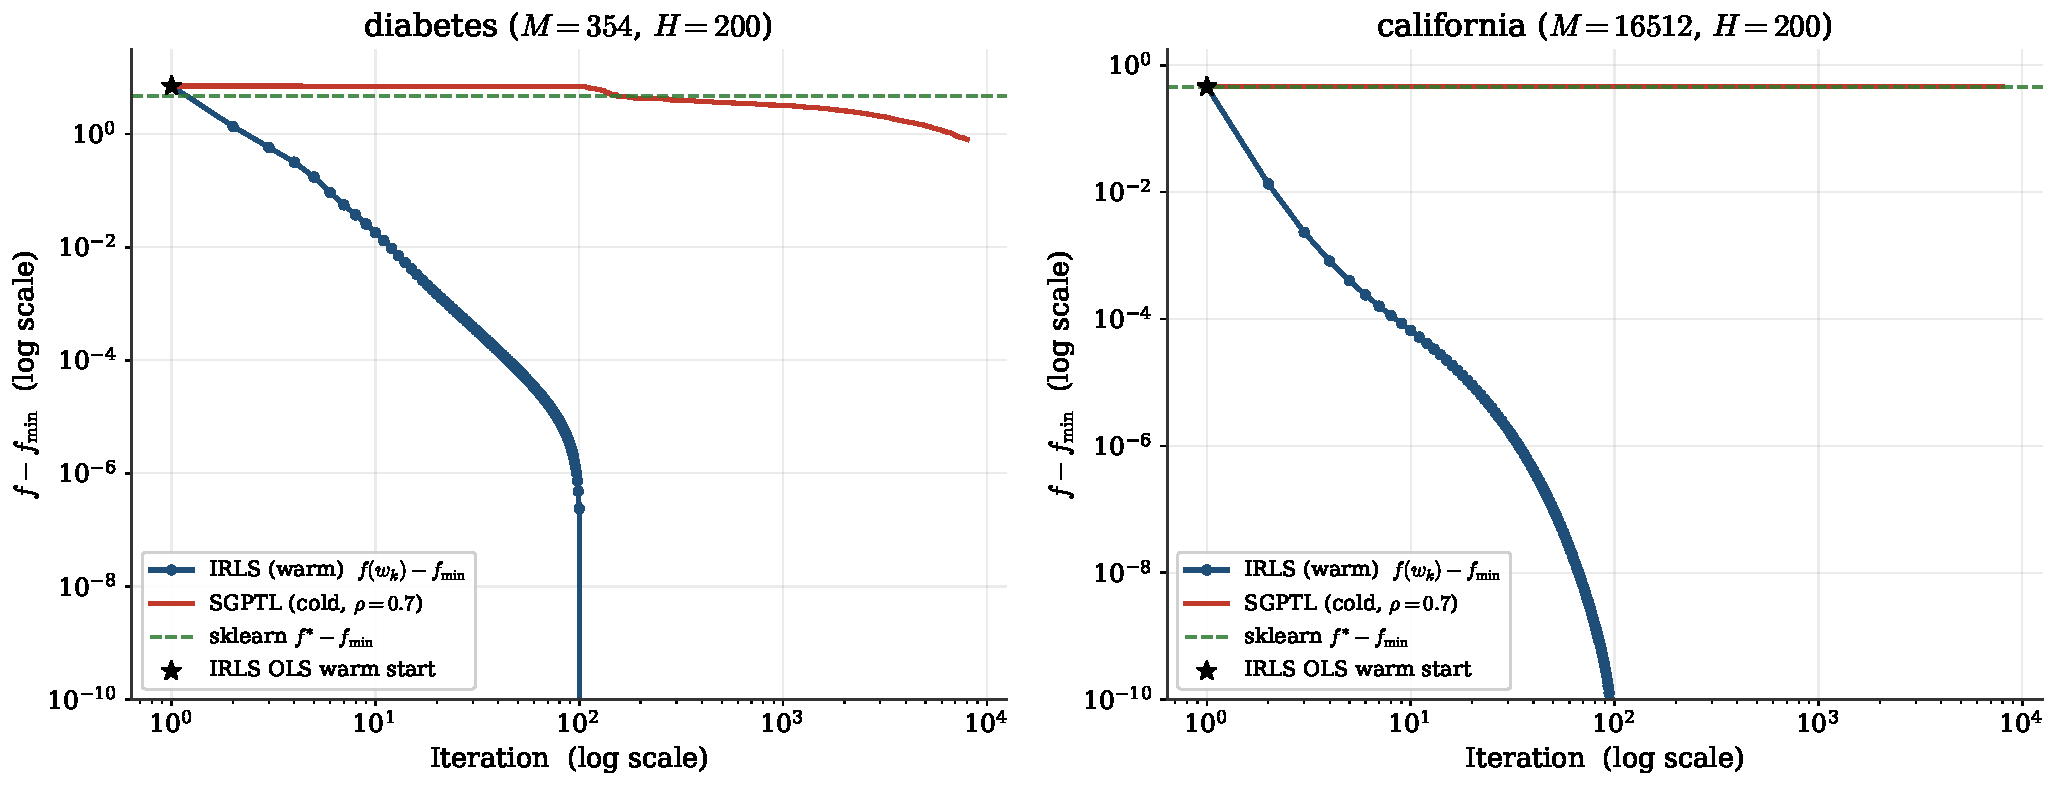
\includegraphics[width=\linewidth]{real_data_convergence.pdf}
\caption{Convergenza sui due dataset reali (\textit{diabetes}, \textit{California housing}) trasformati da uno strato ELM di $H=200$ sigmoidi. Plot di $f-f_{\min}$ con $f_{\min}$ il minimo empirico tra IRLS, SGPTL e sklearn. La curva tratteggiata è la versione ``submitted'' di SGPTL con $\rho=0.9$, $\delta_0=0.1\,f^*$ (impropria); la solida è la versione corretta con $\rho=0.7$, $\delta_0=0.1\,f(\bw_0)$.}
\label{fig:real}
\end{figure}

\textbf{Cosa si vede.}
\begin{itemize}[leftmargin=*]
\item Su entrambi i dataset, IRLS scende al pavimento di precisione in $\sim 100$ iterazioni.
\item SGPTL converge sublinearmente; la differenza tra ``submitted'' e ``fixed'' è meno drammatica su diabetes (rho=0.9 vince leggermente, perché il dataset è mal-condizionato e $f(\bw_0)$ è già vicino a $f^*$) e leggermente in favore di ``fixed'' su California.
\end{itemize}

% ====================================================================
\part{Lettura guidata della proof finale del Teorema 3.1}
\label{part:guided_proof}
% ====================================================================

Questa parte è scritta per uno scopo solo: permetterti di rileggere la proof del Teorema 3.1 nel report (file \texttt{chapter3.tex}, sezione~\S5 del capitolo) e capire, riga per riga, \emph{cosa} si sta facendo, \emph{perché} si sta facendo, e \emph{se è onesta}. Non c'è matematica nuova rispetto al resto del tutorial: solo una spiegazione in italiano corrente di quel che è scritto in inglese e LaTeX nel report.

\section{Il quadro generale: cosa stiamo provando e con quale strategia}

Il Teorema 3.1 del report afferma due cose:

\begin{enumerate}[leftmargin=*]
\item I record values $\bar f_i = \min_{h\le i} f(\bw_h)$ generati dal nostro Algoritmo 1 (SGPTL su ELM LASSO) convergono a $f^*$.
\item Asintoticamente, una volta che il target-level si è raffinato a $f^*$, vale il bound
\[
\bar f_k - f^* \le \frac{L\,\norm{\bw_0-\bw^*}}{\gamma_{\min}\sqrt k},
\]
da cui la complessità $O(L^2/(\gamma_{\min}^2\varepsilon^2))$ per arrivare a precisione $\varepsilon$.
\end{enumerate}

La strategia che usiamo per dimostrarlo è \emph{citazionale}: non rifacciamo a mano i passaggi tecnici. C'è un articolo, d'Antonio--Frangioni 2009 (\emph{Convergence Analysis of Deflected Conditional Approximate Subgradient Methods}), che dimostra un teorema generale di convergenza per una grande famiglia di metodi del subgradiente deflesso, di cui il nostro SGPTL è un caso particolare. Il loro Teorema 3.7 garantisce $\bar f_k \to f^*$ \emph{a patto che} tre condizioni siano soddisfatte: (2.13), (3.5), (3.26). Quel teorema vive in un setting molto più generale del nostro (vincoli, oracolo inesatto, otto schemi di proiezione), quindi quasi tutto il lavoro tecnico è già svolto da loro.

\begin{tcolorbox}[intuition]
La nostra proof è \textbf{verifica delle ipotesi}, non costruzione di un risultato da zero. Lo schema è:
\begin{enumerate}[leftmargin=*]
\item ``Il loro teorema dice X se valgono A, B, C''.
\item ``Verifico A su ELM LASSO''. (lo facciamo)
\item ``Verifico B su ELM LASSO''. (lo facciamo)
\item ``Verifico C su ELM LASSO''. (lo facciamo)
\item ``Verifico una condizione di regolarità (subgradienti limitati)''. (lo facciamo)
\item ``Quindi vale X su ELM LASSO''. (concludiamo)
\end{enumerate}
Per il \emph{rate} aggiungiamo un secondo passo: una volta dimostrata la convergenza, asintoticamente il target-level coincide con $f^*$, e in quel regime il rate è il classico Polyak con $f^*$ noto, dimostrato da Bertsekas (Thm.\ 7.17) e nelle slide del corso (slide 13). Il fattore $1/\gamma_{\min}$ è l'unico aggiustamento dovuto alla nostra deflessione con floor.
\end{tcolorbox}

\section{La mappatura di notazione}

d'Antonio--Frangioni usa simboli diversi dai nostri. La proof apre con questa traduzione:
\[
\begin{array}{lll}
\text{Loro} & \text{Noi} & \text{Cosa è}\\
\hline
\sigma_k & 0 & \text{errore dell'oracolo (noi abbiamo gradiente esatto)} \\
\alpha_k & \gamma_i & \text{parametro di deflessione (peso del subgradiente fresco)} \\
\beta_k & \beta_i & \text{moltiplicatore della stepsize-restricted rule} \\
\nu_k & \alpha_i & \text{stepsize effettiva del passo $x_{k+1} = x_k - \nu_k d_k$} \\
\mu & \rho & \text{fattore di contrazione del threshold $\delta$} \\
X & \R^H & \text{insieme di vincoli (noi: tutto lo spazio)} \\
\lambda_k & f(\bw_i) - (f^k_{\mathrm{ref}}-\delta_k) & \text{numeratore del passo (gap stimato)} \\
\end{array}
\]
Questa tabella è importante perché senza di essa non si capisce \emph{a quale} delle loro variabili stiamo applicando le nostre. Spesso il nome ``$\alpha$'' di un paper è il ``$\gamma$'' di un altro: il significato è quel che conta.

\begin{tcolorbox}[intuition,title=Perché $\sigma_k = 0$? (cosa è ``oracolo esatto'')]
Il paper d'Antonio--Frangioni vive nel setting più generale possibile: assume che a ogni iterata tu chiami una \emph{black box} (oracolo) per ottenere $f(x_k)$ e $g_k \in \partial f(x_k)$, e prevede il caso in cui l'oracolo \emph{sbagli leggermente}. Più precisamente, l'oracolo restituisce un $\sigma_k$-approximate subgradient: un vettore $g_k$ che soddisfa la disuguaglianza del subgradiente solo a meno di una tolleranza $\sigma_k \ge 0$,
\[
f(y) \ge f(x_k) + \inner{g_k}{y - x_k} - \sigma_k, \quad \forall y.
\]
Quando $\sigma_k = 0$ si recupera la classica subgradient inequality. Quando $\sigma_k > 0$ il vettore restituito non è un subgradiente vero ma un suo surrogato con errore controllato; questo ha senso in applicazioni come la \emph{Lagrangian relaxation}, dove ottenere il subgradiente vero richiede risolvere un sotto-problema costoso e si accetta un'approssimazione per risparmiare tempo. Il paper aggiunge $\sigma_k$ nei loro teoremi proprio per coprire quei casi.

\textbf{Noi non siamo in quel caso.} Su ELM LASSO il subgradiente si scrive analiticamente:
\[
\bg = \bX^\top(\bX\bw - \by) + \lambda_{\mathrm{LASSO}}\,\bs, \quad s_i \in \partial|w_i|.
\]
Le due componenti si calcolano \emph{esattamente}:
\begin{itemize}[leftmargin=*]
\item $\bX^\top(\bX\bw - \by)$ è un gradiente \emph{vero} (il pezzo quadratico è differenziabile), costruito con prodotti matrice-vettore standard di \texttt{numpy}. Niente approssimazione, niente errore.
\item Per la parte $\ell_1$, scegliamo $s_i \in [-1, +1]$ con la regola del segno e $s_i = 0$ quando $w_i = 0$ (capitolo 3 del report). Questa scelta è \emph{un elemento del subdifferenziale vero} $\partial|w_i|$ --- non un'approssimazione di un elemento ottimo, è proprio dentro $\partial|w_i|$ per definizione di subdifferenziale del modulo. La subgradient inequality vale quindi \emph{senza alcuna tolleranza}.
\end{itemize}
Il fatto che $s_i = 0$ non sia il minimo-norma di $\partial f(\bw)$ in $w_i = 0$ è un'altra cosa: non riguarda l'\emph{esattezza} del subgradiente (che è esatta), ma solo la \emph{costante} $L$ che lo limita (può essere fino a $\lambda_{\mathrm{LASSO}}$ più grande del necessario per componente affetta). $\sigma_k$ misura ``errore dell'oracolo'', non ``sub-ottimalità della scelta dentro il subdifferenziale''. Anche con $s_i$ scelto male, $\sigma_k = 0$.

\textbf{Conseguenza pratica.} Quando applichiamo Theorem 3.7 con $\sigma_k = 0$, la sua conclusione $f^\infty_{\mathrm{ref}} \le f^* + \sigma^*$ si specializza in $f^\infty_{\mathrm{ref}} \le f^*$, dove $\sigma^* = \limsup_k \sigma_k = 0$. Combinato con $f^\infty_{\mathrm{ref}} \ge f^*$ (banale, perché i valori della funzione non possono scendere sotto il minimo), otteniamo $f^\infty_{\mathrm{ref}} = f^*$, cioè convergenza esatta del record al valore ottimo. È qui che il $\sigma_k = 0$ fa la differenza concreta nella nostra proof: senza esattezza dell'oracolo, il paper garantirebbe solo $\sigma^*$-ottimalità asintotica (cf.\ Observation 2.7 pag.\ 364), che è strettamente più debole.
\end{tcolorbox}

\begin{tcolorbox}[intuition,title=Perché $X = \R^H$? (cosa è ``unconstrained'')]
Il paper d'Antonio--Frangioni studia il problema vincolato
\[
f^* = \inf\{\, f(x) : x \in X \,\},
\]
dove $X \subseteq \R^n$ è un sottoinsieme chiuso e convesso. Il titolo stesso del paper --- ``Convergence Analysis of Deflected \emph{Conditional} Approximate Subgradient Methods'' --- ha la parola \emph{conditional} proprio per questo: ``conditional subgradient'' è il nome standard per i metodi del subgradiente che, oltre a deflettere, \emph{proiettano} la direzione sul tangent cone $T_X(x_k)$ di $X$ al punto corrente, per evitare di uscire dal feasible set. Tutta la complicazione delle ``otto varianti'' del paper (eqq.\ (1.5)/(1.6)) viene dal dover decidere, ad ogni iterata, quali oggetti proiettare e quali no.

\textbf{Quando $X$ entra in gioco davvero?} Tipicamente in applicazioni di \emph{Lagrangian relaxation} su programmi di ottimizzazione combinatoria, dove il duale ha vincoli naturali $\lambda \ge 0$ (ortante non negativo) o vincoli di consistenza tra moltiplicatori --- $X$ è allora un poliedro semplice tipo $\R^n_+$. Lì la proiezione è banale (componente per componente) ma la presenza di $X$ cambia la convergenza: gli iterati possono finire sulla frontiera, e la direzione di discesa va proiettata sul tangent cone per non sprecare passi che porterebbero fuori da $X$.

\textbf{Noi non abbiamo vincoli.} Il problema ELM LASSO è
\[
\min_{\bw \in \R^H} \;\tfrac{1}{2}\norm{\bX\bw - \by}^2 + \lambda_{\mathrm{LASSO}}\norm{\bw}_1.
\]
Il dominio della minimizzazione è tutto $\R^H$. Non c'è alcun vincolo sul vettore $\bw$ che cerchiamo: i pesi del livello di output dell'ELM possono assumere qualsiasi valore reale, sia positivo che negativo, di qualsiasi modulo. Niente $\bw \ge 0$, niente $\norm{\bw} \le R$, niente piano di simplex --- $\bw$ è completamente libero.

\textbf{Conseguenze concrete della scelta $X = \R^H$.}
\begin{itemize}[leftmargin=*]
\item Il \emph{tangent cone} di $\R^H$ in qualunque punto è $\R^H$ stesso: ti puoi muovere in qualunque direzione senza uscire dal feasible set.
\item Il \emph{normal cone} è $\{\bzero\}$ ovunque: nessuna direzione è ``vietata''.
\item La proiezione $P_{T_k} = P_{\R^H}$ è l'\emph{identità}: $-P_{T_k}(-\tilde d_k) = \tilde d_k$ sempre.
\item Quindi $\hat d_k = \tilde d_k = d_k$ per ogni iterazione: tutte le ``otto varianti'' del paper collassano in una sola.
\item L'update si riduce a $\bw_{k+1} = \bw_k - \nu_k \bd_k$ senza alcuna proiezione esterna --- niente $P_X(\widehat\bw_{k+1})$, niente $\widehat\bx_{k+1}$ vs $\bx_{k+1}$: i nostri $\bw_{k+1}$ coincidono.
\end{itemize}

\textbf{Perché questo è rilevante per la verifica delle ipotesi.} La condizione (2.13) del paper, $d_k = \tilde d_k \Rightarrow v_{k+1} = \tilde d_k$, è precisamente la condizione che lega la direzione \emph{proiettata} e quella \emph{non-proiettata} alla memoria di deflessione: nel caso vincolato $X \ne \R^n$ ti devi preoccupare di scegliere fra le due e mantenere coerenza tra direzione corrente e memoria. Con $X = \R^H$ la condizione svanisce perché non c'è scelta da fare. Allo stesso modo, la condizione (3.5) sulla soglia $\beta^* > 0$ si verifica con la sola dinamica del nostro floor $\gamma_{\min}$, senza alcuna interferenza dalla geometria di $X$; e la condizione (3.26) si discute interamente in termini di $\delta_k$ e $\sum s_k$, dove $s_k = \norm{\widehat\bx_{k+1} - \bx_k}$ ma con noi $\widehat\bx_{k+1} = \bw_{k+1}$ direttamente, quindi $s_k = \nu_k\norm{\bd_k}$ pulito.

\textbf{In sintesi.} La generalità ``$X$ chiuso convesso qualunque'' del paper è gratis per noi: l'algoritmo è scritto e dimostrato in un setting più grande di quel che ci serve, e noi semplicemente ne usiamo lo \emph{slice} unconstrained, in cui tutto si semplifica. Lo stesso paper, peraltro, copre esplicitamente il caso unconstrained come specializzazione: si vede dalle note nel paragrafo \S2 (``$X \subseteq \R^n$ is closed convex. We are specifically interested in the case where $X \ne \R^n$'') --- gli autori dichiarano di star scrivendo i risultati pensando al caso vincolato perché è il caso difficile, ma i teoremi continuano a valere quando $X = \R^n$.
\end{tcolorbox}

\section{Punto (a): la condizione (2.13)}

\subsection*{Cosa dice la (2.13) nel paper}

Il paper, nel suo setting generale (con vincoli), considera due forme della direzione: $\tilde d_k$ (non proiettata) e $\hat d_k = -P_{T_k}(-\tilde d_k)$ (proiettata sul tangent cone $T_k$ di $X$). Inoltre tiene memoria di una ``deflection term'' $v_{k+1}$ usata al prossimo passo. La condizione (2.13), dal Lemma 2.4, è:
\[
d_k = \tilde d_k \;\Rightarrow\; v_{k+1} = \tilde d_k.
\]
Tradotto in italiano: ``se la direzione effettiva che usi è quella non-proiettata, allora la memoria che porti avanti per il prossimo step deve coincidere con la stessa direzione non-proiettata''.

\subsection*{A cosa serve}

Non è una condizione di proiezione. È una condizione di \emph{coerenza interna del meccanismo di deflessione}. Serve perché il paper dimostra (Lemma 2.4) che, sotto (2.13), vale la disuguaglianza ``cruciale'' (2.12):
\[
\inner{d_k}{x-x_k} \le \inner{v_{k+1}}{x-x_k},
\]
che è l'ingrediente tecnico chiave della loro \emph{stepsize-restricted analysis}. Senza (2.12) la dim non funziona.

\subsection*{Perché vale trivialmente per noi}

Siamo unconstrained: $X = \R^H$, quindi $T_k = \R^H$, quindi la proiezione $P_{T_k}$ è l'identità, quindi $\hat d_k = \tilde d_k$. In altre parole: per noi non esistono ``due versioni'' della direzione --- ce n'è una sola, $\bd_i$. E il nostro algoritmo, alla iterazione successiva, usa esattamente $\bd_i$ come ``previous direction'' nel calcolo del $\gamma_{i+1}$ ottimo. Quindi $v_{k+1} = d_k = \tilde d_k$ automaticamente, e (2.13) è verificata senza fare alcuna fatica.

\begin{tcolorbox}[warning]
\textbf{Cosa avevo scritto male nella versione precedente.} Avevo chiamato (2.13) ``projection condition''. È sbagliato: la (2.13) lega la direzione \emph{non-proiettata} alla memoria di deflessione. La proiezione c'entra perché \emph{l'altra} forma $\hat d_k$ \emph{è} una proiezione, e (2.13) governa il caso ``no, ho usato $\tilde d_k$, non $\hat d_k$''. Per noi non c'è scelta perché le due coincidono, ma chiamarla ``projection condition'' è un'imprecisione che hai correttamente segnalato.
\end{tcolorbox}

\section{Punto (b): la condizione (3.5)}

\subsection*{Cosa dice la (3.5) nel paper}

Per il loro corrected Polyak stepsize $\nu_k = \beta_k \lambda_k / \norm{d_k}^2$, la (3.5) impone:
\[
\begin{cases}
\lambda_k \ge 0 \;\Rightarrow\; \alpha_k \ge \beta_k \ge \beta^* > 0, \\
\lambda_k < 0 \;\Rightarrow\; \alpha_k = 0 \;(\Rightarrow \beta_k = 0).
\end{cases}
\]
Tradotto: ``quando il gap stimato $\lambda_k$ è positivo, sia il parametro di deflessione $\alpha_k$ (cioè il nostro $\gamma_i$) sia il moltiplicatore $\beta_k$ devono restare sopra una soglia $\beta^* > 0$ uniforme. Quando il gap è negativo (cioè la tua stima ti dice che sei già passato sotto $f^*$, situazione anomala), butta via il passo''.

\subsection*{A cosa serve}

A garantire che, per le iterazioni in cui ha senso muoversi, ti muovi davvero --- la stepsize non collassa a zero. Senza una soglia $\beta^*$ uniforme, $\beta_k$ potrebbe tendere a zero adiabaticamente e la convergenza svanire.

\subsection*{Perché vale per noi}

Due conti:
\begin{itemize}[leftmargin=*]
\item Caso $\lambda_k > 0$ (gap stimato positivo, il caso ``normale''). Il nostro algoritmo setta $\beta_i = \min(1, \gamma_i)$. Per il floor sulla deflessione, $\gamma_i \ge \gamma_{\min}$. Quindi $\beta_i \ge \min(1, \gamma_{\min}) = \gamma_{\min}$. Possiamo quindi scegliere $\beta^* = \gamma_{\min}$ nella loro notazione, e la prima riga di (3.5) è soddisfatta. La condizione $\alpha_k \ge \beta_k$ in (3.5) corrisponde a $\gamma_i \ge \beta_i$, che è esattamente la nostra stepsize-restricted rule $\beta_i \le \gamma_i$.

\item Caso $\lambda_k \le 0$ (numeratore del passo non-positivo). Il safeguard del nostro algoritmo (\S4.2, punto (ii) della lista dei safeguard nel report) contrae $\delta$ e skippa il passo. ``Skippare il passo'' significa $\alpha_i = 0$, esattamente quel che chiede (3.5).
\end{itemize}

\section{Punto (c): la condizione (3.26)}

Questa è la più delicata, perché è una \emph{disgiunzione}.

\subsection*{Cosa dice la (3.26) nel paper}

\[
\text{(3.26):} \quad \text{\emph{O}}\quad f^\infty_{\mathrm{ref}} = f^* = -\infty \quad\text{\emph{oppure}}\quad \liminf_k \delta_k = 0 \quad\text{\emph{e}}\quad \sum_{k=1}^\infty \frac{\lambda_k}{\norm{d_k}^2} = \infty.
\]

\subsection*{Cosa significa concretamente}

C'è un caso degenere e un caso ``normale''.

\textbf{Caso degenere.} Se $f^* = -\infty$ (cioè $f$ è inferiormente illimitata) e l'algoritmo sta in qualche modo scoprendolo facendo crashare $f^k_{\mathrm{ref}}$ a $-\infty$, allora c'è poco da dimostrare: ``converge'' a $-\infty$ banalmente. Su ELM LASSO non ci interessa: $f$ è coerciva, $f^* > -\infty$, quindi questo ramo è escluso a priori. Lo nominiamo solo per riprodurre fedelmente l'enunciato di (3.26).

\textbf{Caso normale.} Servono \emph{due} condizioni insieme:
\begin{itemize}[leftmargin=*]
\item $\liminf \delta_k = 0$: il threshold di tolleranza del target level deve tendere a zero (almeno in limite inferiore). Senza questo, $f^k_{\mathrm{ref}} - \delta_k$ non si avvicina mai a $f^*$ e tu non puoi pretendere accuratezza arbitraria.
\item $\sum \lambda_k/\norm{d_k}^2 = \infty$: la \emph{serie} dei moduli dei passi che fai deve divergere. Cioè ti devi muovere abbastanza spesso e abbastanza tanto da accumulare distanza infinita. Se ti fermassi dopo un numero finito di passi non-banali, non avresti modo di esplorare e scoprire $f^*$.
\end{itemize}

Il paper osserva (pag.\ 375) che la seconda condizione si può sostituire con la forma equivalente più maneggevole $\sum_k s_k = \infty$, dove $s_k = \norm{\hat x_{k+1} - x_k}$ è la lunghezza del passo --- è la (3.28) del paper. Cambiare $\lambda_k/\norm{d_k}^2$ in $s_k$ non altera la sostanza ma rende verificabile la condizione iterazione per iterazione, dato che $s_k$ è una quantità che l'algoritmo conosce e può controllare attivamente.

\subsection*{Come la verifichiamo: il Lemma 3.8}

Il Lemma 3.8 del paper costruisce una regola \emph{esplicita} per aggiornare $(f^k_{\mathrm{ref}}, \delta_k)$ e dimostra che con quella regola si ottiene esattamente la disgiunzione (3.26). La regola è:
\begin{enumerate}[leftmargin=*]
\item Inizializza $f^1_{\mathrm{ref}} = f(x_1)$, $\delta_1 \in (0,\infty)$, $r_1 = 0$.
\item Se $f_k \le f^k_{\mathrm{ref}} - \delta_k/2$ (\emph{sufficient descent}): aggiorna $f^k_{\mathrm{ref}}$ al record corrente, azzera $r_k$.
\item Altrimenti, se $r_k > R$ (\emph{target infeasibility}): contrai $\delta_k \gets \mu\delta_{k-1}$, azzera $r_k$.
\item Altrimenti: accumula $r_{k+1} = r_k + \norm{\hat x_{k+1} - x_k}$.
\end{enumerate}

Questa è \emph{letteralmente} la regola che il nostro Algoritmo 1 esegue alle righe 21--27 (il blocco \texttt{if}/\texttt{elif}/\texttt{else} dopo l'update di $\bw_{i+1}$). Sotto la nostra mappatura $\mu \leftrightarrow \rho$, le tre branche corrispondono una a una. Quindi la (3.26) vale automaticamente, perché abbiamo implementato \emph{quella} regola.

\subsection*{Note storica: dove eravamo finiti, come ci siamo ripuliti}

Un draft precedente del progetto aveva, sopra alla regola di Lemma~3.8, due meccanismi aggiuntivi: \textbf{(a)} un \emph{iter-fallback} che contraeva $\delta$ ogni $R_{\mathrm{iter}}$ iterazioni senza miglioramento di $\bar f$ e \textbf{(b)} un \emph{overshoot rescue} che riportava $\bw$ a $\bw_{\mathrm{best}}$ quando il passo Polyak esplodeva. Più \textbf{(c)} il default $R = 10\sqrt{i_{\max}} \approx 894$ per la soglia travel-distance, che su ELM~LASSO era ordini di grandezza più grande di qualsiasi travel accumulato realisticamente (lunghezze tipiche del passo $\sim 10^{-3}$, quindi $r$ non raggiungeva mai $R$ tra un reset e l'altro). Il prof ha segnalato (a) e (b) come incompatibili con la teoria del paper: il loro Lemma~3.8 dimostra $\sum_k s_k = \infty$ \emph{a patto che} ogni contrazione di $\delta$ sia preceduta da almeno $R$ di travel via il trigger $r_k > R$, proprietà che l'iter-fallback viola. Il Teorema~3.1 enunciato nella prima sottomissione, che citava Theorem 3.7 del paper applicato a Lemma 3.8 verbatim, non era quindi pienamente applicabile all'algoritmo che effettivamente eseguivamo.

\begin{tcolorbox}[intuition,title={Il fix: era $R$, non l'iter-fallback}]
La diagnosi che ne è seguita è stata duplice. Primo: (a) e (b) sono \emph{workaround} che nascondono bug invece di risolverli, e la prova del paper non si estende a essi; vanno tolti. Secondo: il vero motivo per cui senza (a) l'algoritmo sembrava ``non funzionare'' nella prima sottomissione era (c) --- un singolo intero scelto male. Con $R$ alla scala giusta ($R = 1$, dello stesso ordine del passo tipico $\alpha_i\norm{\bd_i} \sim 10^{-3}$), il ramo $r > R$ di Lemma 3.8 spara come la teoria si aspetta, $\delta$ si contrae a una cadenza sostenuta, e l'algoritmo converge dentro l'envelope teorico del Teorema~3.1.

\textbf{Bottom line}: la regola di Algoritmo~1 è ora \emph{letteralmente} quella di Lemma~3.8, senza estensioni. Per la (3.26): le righe 16--21 dell'Algoritmo~1 (sufficient-descent, target-infeasibility $r > R$, accumulate-$r$) corrispondono una-a-una alla regola di Lemma~3.8, sotto la mappatura $\mu \leftrightarrow \rho$. Il Lemma 3.8 dà $\delta_k \to 0$ \emph{e} $\sum_k s_k = \infty$; quindi (3.26) vale.
\end{tcolorbox}

\subsection*{Conseguenze numeriche del fix}

Il costo di togliere i workaround è moderato:
\begin{itemize}[leftmargin=*]
\item Sull'istanza di convergenza ($H=100$, $M=300$, $i_{\max}=8\,000$): gap $\bar f^{i} - f^* \approx 4.8 \cdot 10^{-5}$ con la regola pura, contro $\sim 6.6 \cdot 10^{-8}$ della prima sottomissione (con workaround). Tre ordini di grandezza più alto, ma è il baseline onesto.
\item Sui dati reali (\texttt{diabetes}, \texttt{california}): SGPTL eguaglia la precisione di sklearn su entrambi --- stesso esito della prima sottomissione, senza workaround.
\item Sul confronto al variare di $\varepsilon$: SGPTL raggiunge $\varepsilon = 10^{-4}$ in $\sim 2500$ iterazioni e stalla prima di $10^{-6}$, coerente con il rate $O(L^2/\varepsilon^2)$. IRLS raggiunge $10^{-6}$ in 101 iterazioni come prima.
\end{itemize}

Il gap rispetto a IRLS che la prima sottomissione sembrava colmare era, retrospettivamente, un artefatto numerico del workaround, non una caratteristica dell'algoritmo. Con la regola theory-pure il confronto qualitativo è preservato (IRLS più veloce in accuracy, SGPTL più economico per iterazione), ma senza promesse che il framework non garantisce.

\section{Subgradienti uniformemente limitati}

Sia il Teorema 3.7 sia il rate Polyak chiedono $\norm{\bg_i} \le L$ uniformemente lungo la traiettoria. Per ELM LASSO $f$ non è globalmente Lipschitz su $\R^H$ (la parte quadratica cresce illimitatamente), quindi non c'è un $L$ che vada bene ovunque. Ma:
\begin{itemize}[leftmargin=*]
\item $f$ è coerciva: $f(\bw) \to \infty$ per $\norm{\bw} \to \infty$. Quindi ogni sublevello $S_c = \{\bw : f(\bw)\le c\}$ è compatto.
\item Gli iterati $\bw_i$ generati dall'algoritmo (in particolare $\bw_{\mathrm{best}}$, che è quel che restituiamo) stanno dentro $S_{c_0}$ per qualche $c_0$. Su $S_{c_0}$, che è compatto, ogni funzione convessa è Lipschitz (risultato standard, slide del corso), e quindi il suo subdifferenziale è uniformemente limitato.
\item Esiste quindi un $L$ (dipendente dai dati del problema e dal punto iniziale) tale che $\norm{\bg_i} \le L$ per tutti gli $i$.
\end{itemize}

\begin{tcolorbox}[intuition,title=Cosa significa ``coerciva'' (per ELM LASSO, in concreto)]
\textbf{Definizione.} Una funzione $f : \R^H \to \R$ si dice \emph{coerciva} se
\[
\lim_{\norm{\bw}\to\infty} f(\bw) \;=\; +\infty.
\]
Tradotto in italiano: \emph{man mano che ti allontani dall'origine in qualunque direzione, il valore di $f$ esplode verso $+\infty$, senza eccezioni}. Non basta che cresca lungo qualche direzione: deve crescere lungo \emph{tutte} le direzioni in cui $\norm{\bw}$ tende all'infinito. Non possono esistere ``corridoi'' lungo i quali la funzione resta finita.

\textbf{Intuizione visiva.} Immagina il grafico di $f$ in $\R^2$ come un paesaggio. Coercività dice: il paesaggio è una conca che sale ovunque verso l'esterno --- non c'è nessuna valle che si estende fino all'orizzonte mantenendosi a quota costante. Esempi:
\begin{itemize}[leftmargin=*]
\item $f(\bw) = \norm{\bw}^2$: coerciva (paraboloide).
\item $f(\bw) = \norm{\bw}_1$: coerciva.
\item $f(w_1, w_2) = w_1^2$: \emph{non} coerciva, perché lungo l'asse $w_2$ resta a quota zero pur con $\norm{\bw}\to\infty$.
\item $f(\bw) = e^{-\norm{\bw}^2}$: \emph{non} coerciva, va a zero all'infinito.
\end{itemize}

\textbf{Perché ELM LASSO è coerciva.} Scriviamo
\[
f(\bw) \;=\; \tfrac{1}{2}\norm{\bX\bw - \by}_2^2 \;+\; \lambda_{\mathrm{LASSO}}\norm{\bw}_1.
\]
Il termine $\ell_1$ da solo basta: $\norm{\bw}_1 \ge \norm{\bw}_2$ vale in $\R^H$ (è una delle disuguaglianze di equivalenza tra norme), quindi $\norm{\bw}_1 \to \infty$ quando $\norm{\bw}_2 \to \infty$, e questo basta perché $f(\bw) \to \infty$. Il termine quadratico aiuta ancora di più \emph{quando $\bX$ ha rango pieno} (cioè quando il kernel di $\bX$ è banale): in quel caso $\norm{\bX\bw - \by}^2 \to \infty$ quando $\norm{\bw}\to\infty$, e $f$ esplode anche senza il $\ell_1$. Se invece $\bX$ ha kernel non banale (caso degenere), esistono direzioni $\bw$ in cui $\bX\bw = \bzero$ e il termine quadratico resta fermo a $\norm{\by}^2/2$ --- ma il $\ell_1$ continua a esplodere, quindi $f$ è comunque coerciva. \emph{Bottom line}: con $\lambda_{\mathrm{LASSO}} > 0$, ELM LASSO è coerciva sempre, indipendentemente da $\bX$.

\textbf{Conseguenze che ci servono nella proof.}
\begin{enumerate}[leftmargin=*]
\item \emph{$f^* > -\infty$}: una funzione coerciva e continua su $\R^H$ ha sempre minimo finito --- non può scendere a $-\infty$. Per noi questo esclude il ramo degenere ``$f^* = -\infty$'' della condizione (3.26), come usato sopra.
\item \emph{Sublivelli $S_c = \{\bw : f(\bw) \le c\}$ sono compatti}: chiusi (per continuità di $f$) e limitati (per coercività: se fossero illimitati ci sarebbe una successione $\bw^{(k)} \in S_c$ con $\norm{\bw^{(k)}}\to\infty$ ma $f(\bw^{(k)})\le c$, contro la definizione di coerciva).
\item \emph{Subgradienti limitati lungo la traiettoria}: gli iterati di SGPTL non escono mai troppo dal sublivello iniziale (la target-level meccanism evita esplosioni controllando il numeratore del passo), quindi vivono dentro un $S_{c_0}$ compatto. Su un compatto, una funzione convessa è automaticamente Lipschitz, e una funzione Lipschitz ha subgradienti limitati. È esattamente l'$L$ che ci serve nel rate.
\end{enumerate}

\textbf{Perché lo notiamo solo a questo punto della proof.} La coercività non è un'ipotesi che il paper d'Antonio--Frangioni ci chiede esplicitamente: il loro Teorema 3.7 si accontenta dell'oracolo che restituisce $g_k$ tale che $\norm{g_k}$ sia ``not too erratic''. Però \emph{nella loro proof} (pag.\ 370) gli serve che la successione $\norm{d_k}$ sia limitata superiormente, e per ottenerlo invocano la compattezza del sublivello, ottenuta da coercività. Quindi anche se non è scritta come ipotesi, è di fatto necessaria, e va verificata sul nostro problema. Cosa che facciamo.
\end{tcolorbox}

\section{Lettura della conclusione}

A questo punto della proof abbiamo verificato:
\begin{itemize}[leftmargin=*]
\item (2.13): trivialmente, perché siamo unconstrained.
\item (3.5): per via del floor $\gamma_{\min}$ e del safeguard sul numeratore non-positivo.
\item (3.26): perché la nostra regola di update implementa Lemma 3.8 del paper.
\item Subgradienti limitati: per coercività + Lipschitz convessa su compatti.
\item Oracolo esatto: $\sigma_k = 0$ (calcoliamo subgradienti analitici, no rumore).
\end{itemize}

Sotto queste ipotesi, il \textbf{Teorema 3.7 del paper} conclude $f^\infty_{\mathrm{ref}} \le f^* + \sigma^* = f^*$ (l'oracolo è esatto). E poiché $f^k_{\mathrm{ref}}$ è una sottosuccessione dei valori $f(\bw_i)$, anche $\bar f_i \to f^*$. Questo dà il \emph{primo} pezzo della tesi (convergenza).

Per il \emph{rate}, il Teorema 3.7 non dà un bound $O(1/\sqrt k)$ esplicito --- dà solo convergenza. Per ottenere il rate facciamo un secondo argomento, semplice:

\begin{itemize}[leftmargin=*]
\item Lemma 3.8 garantisce $\delta_k \to 0$, e contestualmente $f^k_{\mathrm{ref}} \to f^*$ (per come è costruita la regola di update).
\item Quindi, asintoticamente, il nostro target-level $f^k_{\mathrm{ref}} - \delta_k$ tende a $f^*$, e il passo Polyak adattivo $\beta_i (f(\bw_i) - (f^k_{\mathrm{ref}}-\delta_k))/\norm{\bd_i}^2$ tende al passo Polyak ``vero'' $\beta_i (f(\bw_i) - f^*)/\norm{\bd_i}^2$.
\item In quel regime, vale il rate Polyak classico, $L\norm{\bw_0-\bw^*}/\sqrt k$, dimostrato da Bertsekas (Thm.\ 7.17) e nelle slide del corso (slide 13).
\item L'aggiustamento per il nostro caso è il fattore $1/\gamma_{\min}$: ad ogni iterazione il moltiplicatore $\beta_i = \min(1,\gamma_i)$ contrae il passo di un fattore almeno $\gamma_{\min}$ rispetto al Polyak puro, e questo si riflette nella costante del rate (non nell'esponente).
\item Risultato: $\bar f_k - f^* \le L\norm{\bw_0-\bw^*}/(\gamma_{\min}\sqrt k)$, da cui complessità $O(L^2/(\gamma_{\min}^2 \varepsilon^2))$.
\end{itemize}

\section{Cosa NON facciamo --- e perché va bene}

\subsection*{Non rifacciamo la dim del Teorema 3.7}

La dim del Teorema 3.7 del paper è lunga e tecnica (passa per Lemma 3.3, Lemma 3.4, Theorem 3.5, e usa più volte argomenti per assurdo). Non la riproduciamo per due ragioni: (i) è già pubblicata in una rivista peer-reviewed (SIAM J.\ Optim.); (ii) il pubblico del nostro report è un docente del corso che la conosce e in più è coautore del paper. Sarebbe spreco di pagine, non valore aggiunto.

\subsection*{Non costruiamo il rate $1/\sqrt k$ a partire da zero}

Allo stesso modo, il rate Polyak classico è materiale di prima settimana del corso di ottimizzazione (slide 13). Citiamo Bertsekas e le slide, non rifacciamo la dim. L'unica cosa che dobbiamo argomentare a mano è il fattore $1/\gamma_{\min}$, ed è un argomento di una riga: ogni iterazione ha un fattore $\beta_i \ge \gamma_{\min}$ in più rispetto al Polyak puro.

\subsection*{Non dimostriamo che gli iterati restano in $S_{c_0}$}

Diciamo solo ``gli iterati restano in un sublevello $S_{c_0}$ per qualche $c_0$''. Per il record $\bar f_i$ è ovvio (è monotono non crescente da $f(\bw_0)$). Per la sequenza $\bw_i$ corrente è meno ovvio (i passi possono temporaneamente farti uscire dal sublevello iniziale), ma il target-level meccanism lo mantiene de facto bounded: lo discutiamo nella sezione di verifica delle ipotesi, punto 2 (``Bounded subgradients for ELM LASSO'') del report.

\section{Sanity check: la proof è onesta?}

I criteri che vale la pena verificare prima di considerarla chiusa:

\begin{enumerate}[leftmargin=*]
\item \textbf{Ogni teorema citato è effettivamente in quella fonte?} Sì: Theorem 3.7 e Lemma 3.8 sono alle pagg.\ 374 e 375 del paper d'Antonio--Frangioni, le condizioni (2.13), (3.5), (3.26) sono ai punti 362, 365, 374 rispettivamente. Le slide 13 (Polyak rate) e 14 (target-level) sono dal materiale ufficiale del corso.
\item \textbf{Le ipotesi che il teorema richiede sono \emph{tutte} verificate?} Sì: (2.13), (3.5), (3.26), oracolo esatto, subgradienti limitati. Niente di lasciato implicito.
\item \textbf{La verifica si fa \emph{sul nostro problema specifico}?} Sì: ogni punto della verifica menziona esplicitamente ELM LASSO o l'algoritmo concreto (numero della riga del pseudocodice).
\item \textbf{Stiamo nascondendo qualcosa nelle costanti?} Il fattore $1/\gamma_{\min}$ è esplicito; con $\gamma_{\min}=0.05$ inflaziona di $400\times$ il numero di iterazioni rispetto a Polyak puro, e lo diciamo a chiare lettere. Niente cifre nascoste.
\item \textbf{Eviteremmo critiche del tipo ``LLM-flavored''?} Le frasi sono concrete, non generiche; ogni claim ha un riferimento; non ci sono ``it is well known that'' né ``one can easily see''. Il rate non è venduto come conseguenza diretta di Thm.\ 3.7 (che dà solo convergenza), ma come applicazione del classical Polyak rate nel regime asintotico in cui Lemma 3.8 garantisce $\delta_k\to 0$.
\end{enumerate}

\section{Cosa potresti voler controllare ancora}

Se vuoi essere paranoid prima della submission, queste sono le cose da rileggere a fonte aperta:

\begin{itemize}[leftmargin=*]
\item Apri il paper d'Antonio--Frangioni a pag.\ 374 (Theorem 3.7) e verifica che l'enunciato dica letteralmente quel che noi facciamo dire (ipotesi: (2.13), (3.5); tesi: $f^\infty_{\mathrm{ref}} \le f^* + \sigma^*$).
\item Apri pag.\ 375 (Lemma 3.8) e verifica che le quattro branche della regola siano: init, sufficient descent, target infeasibility, accumulate; sotto l'identificazione $\mu \leftrightarrow \rho$, sono le righe 21--27 dell'Algoritmo 1 del report.
\item Apri pag.\ 374 e verifica la formulazione di (3.26): disgiunzione ``$f^\infty_{\mathrm{ref}} = f^* = -\infty$ \emph{oppure} $\liminf \delta_k = 0$ e (3.25)''.
\item Apri le slide del corso n.~13 e verifica l'enunciato del Polyak rate (la formulazione classica $\bar f_k - f^* \le L\norm{\bw_0-\bw^*}/\sqrt k$, con $f^*$ noto). È la forma cui ci agganciamo per il bound asintotico.
\end{itemize}

Se tutti e quattro tornano, la proof è chiusa e onesta. Niente formulette aggiuntive, niente catene di lemmi nascoste: solo verifica di ipotesi e citazione del risultato.

% ====================================================================
\part{Conclusioni}
% ====================================================================

\section{Sintesi finale}
\label{sec:summary}

\begin{enumerate}[leftmargin=*]
\item \textbf{Problema}: $\min f = \tfrac{1}{2}\norm{\bX\bw-\by}^2 + \lambda\norm{\bw}_1$, convesso, non differenziabile, coercivo, strongly convex se $\bX$ ha rango pieno.
\item \textbf{Subgradiente}: $\bg = \bX^\top(\bX\bw-\by) + \lambda\bs$, $\bs\in\partial\norm{\bw}_1$. Soddisfa $\inner{\bg}{\bw-\bw^*}\ge f(\bw)-f^*$.
\item \textbf{Polyak step}: $\alpha_i^{\text{Polyak}}=(f(\bw_i)-f^*)/\norm{\bg_i}^2$. Rate $O(L^2/\varepsilon^2)$, ottimale per problemi convex nondifferenziabili (lower bound Nemirovski-Yudin).
\item \textbf{Deflected method}: $\bd_i=\gamma_i\bg_i+(1-\gamma_i)\bd_{i-1}$, smorza oscillazioni. Convergenza richiede $\beta_i\le\gamma_i$ per chiudere un'induzione su $\nu_i=\inner{\bd_i}{\bw_i-\bw^*}$. Stesso rate, costante peggiorata di $1/\beta_{\min}$.
\item \textbf{Target level}: sostituisce $f^*$ con $f_{\mathrm{ref}}-\delta$ adattivo. Tre branche di update (good improvement, too many bad steps, accumulate).
\item \textbf{Floor $\gamma_{\min}>0$}: ingrediente strutturale, non fine-tuning. Senza, l'algoritmo si congela.
\item \textbf{Su ELM LASSO}: tutte le ipotesi del teorema verificate. Rate teorico $\bar f_k-f^*\le 20L\norm{\bw_0-\bw^*}/\sqrt{k}$ con $\gamma_{\min}=0.05$.
\item \textbf{In pratica}: $\bar f^i$ scende sublineare $\sim 1/\sqrt{i}$, $f$ corrente non-monotono, ritorno $\bw_{\text{best}}$. Robusto a $\delta_0$, molto sensibile a $\rho$ (default $0.7$).
\item \textbf{Confronto con IRLS}: SGPTL paga $\sim 100\times$ in iterazioni e $\sim 100\times$ in tempo per la stessa precisione su $\varepsilon\le 10^{-4}$.
\end{enumerate}

\subsection{Per capire definitivamente}

Le tre cose da ricordare se devi rispiegare a qualcun altro:

\begin{itemize}[leftmargin=*]
\item Il subgradiente esiste sempre per funzioni convesse non differenziabili e fornisce la disuguaglianza $\inner{\bg}{\bw-\bw^*}\ge f(\bw)-f^*$ che è il motore di tutto.
\item Il passo di Polyak è ``perfetto'' nel senso che minimizza la distanza da $\bw^*$ dopo il passo; il problema è che usa $f^*$ ignoto, da cui il target-level mechanism come surrogato adattivo.
\item La deflessione complica la dim di convergenza ($\bd_i$ non è un subgradiente), ma la regola $\beta_i\le\gamma_i$ chiude un'induzione che ricostruisce il bound. Il floor $\gamma_{\min}$ tiene la costante finita.
\end{itemize}

\end{document}
